%% Hapax: Fusing Dependent Tensor Reductions by Deriving Single-Pass Reducers
%% PLDI 2027 submission (PACMPL, acmsmall). Build: bash build.sh
%% Every number in the text comes from gen/stats.tex (generated from data/*.json);
%% hand-written numbers carry a "% src:" comment.
\PassOptionsToPackage{table}{xcolor}
\documentclass[acmsmall,screen,review,anonymous,nonacm]{acmart}

\citestyle{acmnumeric}
% Packages. acmart already loads amsmath, amsthm, booktabs, natbib, hyperref,
% xcolor, graphicx, caption and microtype: do not load them again.
\usepackage{mathtools}
\usepackage{stmaryrd}            % \llbracket \rrbracket
\usepackage{xspace}
\usepackage{array}
\usepackage{multirow}
\usepackage{subcaption}
\usepackage{wrapfig}
\usepackage{pifont}              % \ding{51} check, \ding{55} cross
\usepackage{listings}
\usepackage{tikz}
\usetikzlibrary{arrows.meta,positioning,fit,calc,backgrounds,shapes.misc,decorations.pathreplacing,patterns}
\usepackage{pgfplots}
\pgfplotsset{compat=1.18}
\usepackage[ruled,linesnumbered,noend]{algorithm2e}
\usepackage{cleveref}            % after hyperref (loaded by acmart)
\crefname{section}{Section}{Sections}
\Crefname{section}{Section}{Sections}
\crefname{figure}{Fig.}{Figs.}
\Crefname{figure}{Figure}{Figures}
\crefname{table}{Table}{Tables}
\crefname{algocf}{Algorithm}{Algorithms}
\crefname{algorithm}{Algorithm}{Algorithms}
\Crefname{algocf}{Algorithm}{Algorithms}
\crefname{lstlisting}{Listing}{Listings}
\crefname{listing}{Listing}{Listings}
\Crefname{listing}{Listing}{Listings}
\crefname{theorem}{Theorem}{Theorems}
\crefname{lemma}{Lemma}{Lemmas}
\crefname{proposition}{Proposition}{Propositions}
\crefname{definition}{Definition}{Definitions}
\crefname{example}{Example}{Examples}
\crefname{corollary}{Corollary}{Corollaries}
\crefname{equation}{Eq.}{Eqs.}
\crefname{appendix}{Appendix}{Appendices}


% Keep half-width diagrams/algorithms beside their explanatory prose without reordering the argument.
\newenvironment{paperdiagram}{\begin{minipage}[t]{0.48\linewidth}\vspace{0pt}}{\end{minipage}}

% Reserve room for a wrapped diagram; its accompanying prose remains pageable.
\newcommand{\reservewrapspace}[1]{%
  \par\penalty-100\relax\begingroup
  \dimen0=#1\relax
  \dimen2=\pagegoal\advance\dimen2 by -\pagetotal
  \ifdim\dimen0>\dimen2\newpage\fi
  \endgroup
}

% Clear any remaining wrapped height before a full-width theorem or display.
% wrapfig counts the remaining narrow lines plus one; clearing alone adds no space.
\newcommand{\finishwrapspace}{%
  \par
  \ifnum\value{WF@wrappedlines}>1\relax
    \vspace{\dimexpr\value{WF@wrappedlines}\baselineskip-\baselineskip\relax}%
  \fi
  \WFclear
}

% Colours: one meaning each, used in figures, equations and captions alike
% (Okabe-Ito, distinguishable in grayscale by the line style that goes with it).
\definecolor{origblue}{HTML}{0072B2}   % the original program, original values
\definecolor{staleorange}{HTML}{D55E00} % stale or wrong values (naive fusion)
\definecolor{fixgreen}{HTML}{009E73}   % values corrected by the derived join
\definecolor{auxpurple}{HTML}{8E5AA8}  % states the program does not compute
\definecolor{boxgray}{HTML}{F2F2F2}
\definecolor{rulegray}{HTML}{8C8C8C}
\definecolor{codebg}{HTML}{F7F7F7}
\definecolor{kwgreen}{HTML}{1B7837}
\definecolor{strred}{HTML}{B2182B}
\definecolor{cmtgray}{HTML}{6E6E6E}

\newcommand{\orig}[1]{\textcolor{origblue}{#1}}
\newcommand{\stale}[1]{\textcolor{staleorange}{#1}}
\newcommand{\fix}[1]{\textcolor{fixgreen}{#1}}
\newcommand{\aux}[1]{\textcolor{auxpurple}{#1}}

% TikZ styles
\tikzset{
  >={Stealth[length=2mm]},
  artifact/.style={draw, rounded corners=2pt, fill=white, font=\sffamily\small,
    inner sep=3pt, align=center},
  stage/.style={draw, rounded corners=2pt, fill=boxgray, font=\sffamily\small,
    inner sep=4pt, align=center, minimum height=7mm},
  future/.style={draw, dashed, rounded corners=2pt, font=\sffamily\small,
    inner sep=4pt, align=center, text=rulegray},
  flow/.style={->, thick, draw=origblue},
  weak/.style={->, densely dashed, draw=rulegray},
  cell/.style={draw, minimum width=7mm, minimum height=6mm, font=\small, inner sep=1pt},
  tmpcell/.style={cell, densely dashed},
  lbl/.style={font=\sffamily\scriptsize, text=cmtgray},
}

% Code listings (TE is Python)
\lstdefinestyle{te}{
  language=Python,
  basicstyle=\ttfamily\scriptsize,
  keywordstyle=\color{kwgreen}\bfseries,
  stringstyle=\color{strred},
  commentstyle=\color{cmtgray},
  morekeywords={te,tir},
  columns=fullflexible,
  keepspaces=true,
  breaklines=true,
  breakatwhitespace=false,
  postbreak=\mbox{\textcolor{rulegray}{$\hookrightarrow$}\space},
  showstringspaces=false,
  frame=tb,
  framerule=0.4pt,
  rulecolor=\color{rulegray},
  aboveskip=2pt,
  belowskip=2pt,
  xleftmargin=2pt,
  numbers=none,
  escapeinside={(*@}{@*)},
}
\lstset{style=te}

% algorithm2e: procedure names in small caps, as in the reference papers
\SetKwProg{Fn}{function}{}{}
\SetFuncSty{textsc}
\SetArgSty{textup}
\DontPrintSemicolon


% Illustrative program forms use the Listing counter, separately from method algorithms.
\lstdefinestyle{pseudocode}{
  style=te,
  language={},
  basicstyle=\small\rmfamily,
  keywordstyle=\bfseries,
  morekeywords={for,return,function},
  mathescape=true,
  captionpos=t,
  numbers=none,
  xleftmargin=0pt,
}

% ---------------------------------------------------------------- names
\newcommand{\sys}{Hapax\xspace}
\newcommand{\Neptune}{Neptune\xspace}
\newcommand{\RedFuser}{RedFuser\xspace}
\newcommand{\TE}{TE\xspace}
\newcommand{\code}[1]{\texttt{\small #1}}
\newcommand{\commreducer}{\code{te.comm\_reducer}\xspace}

% ---------------------------------------------------------------- notation
\newcommand{\Ax}{J}                       % the reduction axis
\newcommand{\pa}{A}                       % parts
\newcommand{\pb}{B}
\newcommand{\dunion}{\uplus}
\newcommand{\st}{I}                       % state map S -> I(S)
\newcommand{\Mrg}{\operatorname{join}}
\newcommand{\ident}{e}
\newcommand{\leaf}{L}
\newcommand{\epi}{E}
\newcommand{\red}{\oplus}
\newcommand{\ctx}{\kappa}
\newcommand{\cnt}{n}
\newcommand{\Judged}{\mathcal{A}}         % the judgement's tuple of reductions
\newcommand{\Own}{\mathcal{B}}            % the program's own loop results
\newcommand{\Cls}[1]{\mathcal{C}_{\mathrm{#1}}}
\newcommand{\R}{\mathbb{R}}
\newcommand{\sem}[1]{\llbracket #1 \rrbracket}
\newcommand{\maxop}{\operatorname{max}}
\newcommand{\Sum}{\textstyle\sum}
\DeclareMathOperator*{\bigred}{\bigoplus}

% ---------------------------------------------------------------- marks
\newcommand{\cmark}{\textcolor{fixgreen}{\ding{51}}}
\newcommand{\xmark}{\textcolor{staleorange}{\ding{55}}}
\newcommand{\pmark}{\textcolor{rulegray}{$\circ$}}       % partial
\newcommand{\nr}{\textcolor{rulegray}{n.r.}}            % not reported
\newcommand{\markRefused}{\textcolor{staleorange}{\ding{55}}}
\newcommand{\markFrontend}{\textcolor{rulegray}{\ding{55}}}
\newcommand{\tagP}{\textsc{p}}            % proven
\newcommand{\tagM}{\textsc{m}}            % measured
\newcommand{\tagS}{\textsc{s}}            % sampled

% ---------------------------------------------------------------- drafting
\newif\ifperf          % \perftrue once GPU numbers exist (Section 8.5, 7.2)
\perffalse
\newif\ifsubmit
\submitfalse
\newcounter{placeholders}
\newcommand{\placeholder}[1]{%
  \stepcounter{placeholders}%
  \ifsubmit\errmessage{placeholder left in a submission build: #1}\fi
  \par\noindent\fcolorbox{staleorange}{white}{\parbox{\dimexpr\linewidth-2\fboxsep-2\fboxrule}{%
    \small\textcolor{staleorange}{\textbf{Placeholder.}} #1}}\par}
\newcommand{\todo}[1]{\textcolor{staleorange}{[\textbf{TODO}: #1]}}

\submitfalse

% generated by Hapax/scripts/gen_tex.py -- do not edit
\newcommand{\dataCommit}{6c46fb1b02\xspace}
%   src: data/fused_ops.json meta.commit
\newcommand{\dataStale}{false\xspace}
%   src: meta.commit of every data/*.json vs HEAD
\newcommand{\pythonVersion}{3.12.14\xspace}
%   src: fused_ops.json meta.python
\newcommand{\sympyVersion}{1.14.0\xspace}
%   src: fused_ops.json meta.sympy
\newcommand{\zThreeVersion}{5.3.3\xspace}
%   src: fused_ops.json meta.z3
\newcommand{\cvcFiveVersion}{1.4.2\xspace}
%   src: fused_ops.json meta.cvc5
\newcommand{\nRegistry}{51\xspace}
%   src: fused_ops.json meta.registry (len(OPERATORS))
\newcommand{\nFusible}{44\xspace}
%   src: fused_ops.json meta.registry_fusible
\newcommand{\nFused}{42\xspace}
%   src: fused_ops.json: rows with fused = true
\newcommand{\nNegative}{7\xspace}
%   src: registry minus fusible
\newcommand{\nChains}{45\xspace}
%   src: fused_ops.json: chains over fused rows
\newcommand{\nPassesBefore}{117\xspace}
%   src: sum of passes_before
\newcommand{\nPassesAfter}{45\xspace}
%   src: sum of passes_after
\newcommand{\nPassesEqualHand}{42\xspace}
%   src: rows with passes_after == passes_hand
\newcommand{\nStates}{162\xspace}
%   src: sum of len(chain.states)
\newcommand{\nDerived}{49\xspace}
%   src: sum of len(chain.auxiliaries)
\newcommand{\nDerivedOps}{26\xspace}
%   src: rows with a non-empty auxiliaries list
\newcommand{\nCountOnlyOps}{0\xspace}
%   src: rows whose only auxiliary is count
\newcommand{\nMoreAuxOps}{26\xspace}
%   src: derived-ops minus count-only
\newcommand{\nNoAuxOps}{16\xspace}
%   src: fused rows without auxiliaries
\newcommand{\nAddedCount}{0\xspace}
%   src: auxiliaries named count
\newcommand{\nAddedR}{34\xspace}
%   src: auxiliaries ending .r<k> (supplemented coefficients)
\newcommand{\nAddedH}{6\xspace}
%   src: auxiliaries ending .h<k> (hoisted coefficients)
\newcommand{\nAddedM}{0\xspace}
%   src: auxiliaries ending .m<k> (parts of a max)
\newcommand{\nSupplement}{43\xspace}
%   src: selection steps with action supplement
\newcommand{\nPromote}{0\xspace}
%   src: selection steps with action promote
\newcommand{\nHoist}{6\xspace}
%   src: selection steps with action hoist
\newcommand{\nParts}{0\xspace}
%   src: selection steps with action parts
\newcommand{\nSplit}{0\xspace}
%   src: selection steps with action split
\newcommand{\nNoStep}{19\xspace}
%   src: chains with no selection step
\newcommand{\nStatesEqualJudged}{45\xspace}
%   src: chains with len(states) == theory_states
\newcommand{\nStatesBelowJudged}{0\xspace}
%   src: chains with len(states) < theory_states
\newcommand{\nStatesAboveJudged}{0\xspace}
%   src: chains with len(states) > theory_states
\newcommand{\nMechRebase}{16\xspace}
%   src: fused rows whose heaviest step is rebase
\newcommand{\nMechSupplement}{20\xspace}
%   src: fused rows whose heaviest step is supplement
\newcommand{\nMechPromote}{0\xspace}
%   src: fused rows whose heaviest step is promote
\newcommand{\nMechParts}{0\xspace}
%   src: fused rows whose heaviest step is parts
\newcommand{\nMechHoist}{6\xspace}
%   src: fused rows whose heaviest step is hoist
\newcommand{\nDomains}{7\xspace}
%   src: info_en.py domains of fused rows, excluding Constructed
\newcommand{\nShowcase}{17\xspace}
%   src: all selected showcase rows, including failures
\newcommand{\nShowFused}{17\xspace}
%   src: successfully fused showcase rows
\newcommand{\ratioCentredMedian}{1.20\xspace}
%   src: median err_synth[0]/err_unfused[0]
\newcommand{\ratioCentredMin}{0.23\xspace}
%   src: min of the same
\newcommand{\ratioCentredMax}{9.7\xspace}
%   src: max of the same
\newcommand{\nRatioCentredLeOne}{20\xspace}
%   src: count ratio_c <= 1
\newcommand{\nRatioCentredLeTwo}{30\xspace}
%   src: count ratio_c <= 2
\newcommand{\nRatioCentredLeFive}{40\xspace}
%   src: count ratio_c <= 5
\newcommand{\nRatioCentred}{42\xspace}
%   src: operators with a centred ratio
\newcommand{\ratioOffsetMedian}{1.06\xspace}
%   src: median err_synth[1]/err_unfused[1] (both > 0)
\newcommand{\ratioOffsetMin}{0.00\xspace}
%   src: min of the same
\newcommand{\ratioOffsetMax}{60.0\xspace}
%   src: max of the same
\newcommand{\nRatioOffset}{40\xspace}
%   src: operators with an offset ratio
\newcommand{\nRatioOffsetLeTen}{36\xspace}
%   src: count ratio_o <= 10
\newcommand{\gateWorstMargin}{0.041\xspace}
%   src: max candidate/bound over families (kurtosis)
\newcommand{\gateWorstOp}{kurtosis\xspace}
%   src: operator with the worst gate margin
\newcommand{\nGateHuge}{10\xspace}
%   src: fused rows gated on the huge family
\newcommand{\nGateTiny}{22\xspace}
%   src: fused rows gated on the tiny family
\newcommand{\nSameAsHand}{6\xspace}
%   src: rows whose synthesised errors equal the hand-written ones (both families)
\newcommand{\varianceOffsetSynth}{$2.9\times10^{-4}$\xspace}
%   src: variance gate offset candidate
\newcommand{\varianceOffsetUnfused}{$1.0\times10^{-6}$\xspace}
%   src: variance gate offset original
\newcommand{\varianceOffsetInherent}{$2.1\times10^{-4}$\xspace}
%   src: variance gate offset inherent
\newcommand{\varianceOffsetBound}{$2.1\times10^{-2}$\xspace}
%   src: 100 max(original, inherent) + 64 u, variance offset
\newcommand{\nPreservingFailures}{2\xspace}
%   src: fused_ops.json rows not fused
\newcommand{\nRegUnknown}{5\xspace}
%   src: registry negatives judged 'no single pass is known'
\newcommand{\nRegRefused}{2\xspace}
%   src: registry negatives refused by the checks
\newcommand{\nRegNotRead}{0\xspace}
%   src: registry negatives with no chain read
\newcommand{\nRegNoSelect}{0\xspace}
%   src: registry negatives where selection failed
\newcommand{\nCollectedOther}{20\xspace}
%   src: unfused.json rows from the survey and extra programs
\newcommand{\nOtherNowFused}{2\xspace}
%   src: of those, fused at HEAD
\newcommand{\nOtherUnknown}{8\xspace}
%   src: survey/extra judged 'no single pass is known'
\newcommand{\nOtherRefused}{5\xspace}
%   src: survey/extra refused
\newcommand{\nOtherNotRead}{5\xspace}
%   src: survey/extra not read or unsupported
\newcommand{\nNeptunePrograms}{15\xspace}
%   src: prior.json rows with paper = Neptune
\newcommand{\nNeptuneFused}{9\xspace}
%   src: Neptune: fused
\newcommand{\nNeptuneFrontend}{5\xspace}
%   src: Neptune: skipped by the frontend
\newcommand{\nNeptuneRefused}{1\xspace}
%   src: Neptune: refused by the checks
\newcommand{\nNeptuneNotChain}{0\xspace}
%   src: Neptune: no single-axis chain
\newcommand{\nRedFuserPrograms}{10\xspace}
%   src: prior.json rows with paper = RedFuser
\newcommand{\nRedFuserFused}{6\xspace}
%   src: RedFuser: fused
\newcommand{\nRedFuserFrontend}{0\xspace}
%   src: RedFuser: skipped by the frontend
\newcommand{\nRedFuserRefused}{1\xspace}
%   src: RedFuser: refused by the checks
\newcommand{\nRedFuserNotChain}{1\xspace}
%   src: RedFuser: no single-axis chain
\newcommand{\nPriorPrograms}{25\xspace}
%   src: prior.json rows
\newcommand{\nPriorFused}{15\xspace}
%   src: prior.json rows fused
\newcommand{\nPriorFrontend}{6\xspace}
%   src: prior.json rows not read
\newcommand{\nPriorRefused}{2\xspace}
%   src: prior.json rows refused
\newcommand{\aOneFused}{not fused\xspace}
%   src: prior.json a1_program a1_numbers.fused
\newcommand{\aOneTruth}{9\xspace}
%   src: prior.json a1_program a1_numbers.truth
\newcommand{\nInvCanonical}{40\xspace}
%   src: proofs_timing.json invariant_proof == canonical
\newcommand{\nInvCaseSplit}{0\xspace}
%   src: invariant_proof == case-split
\newcommand{\nInvSympy}{0\xspace}
%   src: invariant_proof == sympy
\newcommand{\nPrintedChains}{42\xspace}
%   src: chains whose re-based merge printed
\newcommand{\nNotPrintedChains}{3\xspace}
%   src: chains printed in canonical form
\newcommand{\nSlots}{149\xspace}
%   src: printed slots
\newcommand{\nSlotsCanonical}{146\xspace}
%   src: printed slots proven by canonical identity
\newcommand{\nSlotsCaseSplit}{0\xspace}
%   src: printed slots proven by a case split
\newcommand{\nSlotsSympy}{0\xspace}
%   src: printed slots proven by SymPy
\newcommand{\failedSelectMaxMs}{1702\xspace}
%   src: unfused registry candidates: max median selection time, ms
\newcommand{\showOriginalOps}{8\xspace}
%   src: fused_ops.json showcase operators with every chain route = original
\newcommand{\showRebaseOps}{7\xspace}
%   src: fused_ops.json showcase operators with every chain route = rebase
\newcommand{\showSygusOps}{2\xspace}
%   src: fused_ops.json showcase operators with every chain route = sygus
\newcommand{\nShowcaseDomains}{6\xspace}
%   src: info_en.py domains of the showcase rows
\newcommand{\showPassesBefore}{54\xspace}
%   src: showcase: sum of passes_before
\newcommand{\showPassesAfter}{19\xspace}
%   src: showcase: sum of passes_after
\newcommand{\showChains}{19\xspace}
%   src: showcase: chains
\newcommand{\showStates}{72\xspace}
%   src: showcase: states
\newcommand{\showDerived}{19\xspace}
%   src: showcase: auxiliaries
\newcommand{\showDerivedOps}{9\xspace}
%   src: showcase rows with auxiliaries
\newcommand{\showNoStep}{8\xspace}
%   src: showcase rows without a selection step
\newcommand{\showSelectMaxMs}{4045\xspace}
%   src: showcase: max median select time, ms
\newcommand{\showSelectMedianMs}{65\xspace}
%   src: showcase: median of median select times, ms
\newcommand{\showFuseSinkhorn}{4.2\xspace}
%   src: showcase: sinkhorn_iteration median fuse time, s
\newcommand{\showFuseMax}{13.08\xspace}
%   src: accepted showcase: max median fuse time, s
\newcommand{\showFuseMedian}{0.25\xspace}
%   src: accepted showcase: median fuse time, s
\newcommand{\showJudgeMaxMs}{13.4\xspace}
%   src: showcase: max median judge time, ms
\newcommand{\showInvCanonical}{16\xspace}
%   src: showcase: invariants proven by canonical identity
\newcommand{\showRatioLeOne}{9\xspace}
%   src: showcase: centred ratio <= 1
\newcommand{\showGateWorstMargin}{0.041\xspace}
%   src: showcase: worst candidate/bound
\newcommand{\timeJudgeMaxMs}{13.4\xspace}
%   src: max median judge time, ms
\newcommand{\timeJudgeMedianMs}{3.2\xspace}
%   src: median of median judge times, ms
\newcommand{\timeSelectMedianMs}{49\xspace}
%   src: median of median select times, ms
\newcommand{\timeSelectMaxMs}{4045\xspace}
%   src: max median select time, ms
\newcommand{\timeFuseMedian}{0.23\xspace}
%   src: median fuse time, s
\newcommand{\timeFuseMin}{0.11\xspace}
%   src: min fuse time excluding the two Sinkhorn iterations, s
\newcommand{\timeFuseMax}{13.08\xspace}
%   src: max fuse time excluding the two Sinkhorn iterations, s
\newcommand{\timeFuseSinkhorn}{4.2\xspace}
%   src: max fuse time of the two Sinkhorn iterations, s
\newcommand{\nTimeRest}{42\xspace}
%   src: operators other than the two Sinkhorn iterations
\newcommand{\timeSelectMaxOp}{papr\xspace}
%   src: operator with the slowest selection
\newcommand{\timeSelectKurtosisMs}{158\xspace}
%   src: kurtosis median select time, ms
\newcommand{\timeFuseKurtosis}{0.38\xspace}
%   src: kurtosis median fuse time, s
\newcommand{\hazProjUnfused}{$2.5\times10^{-6}$\xspace}
%   src: hazards.json projection unfused
\newcommand{\hazProjSynth}{$8.8\times10^{-3}$\xspace}
%   src: hazards.json projection synthesised
\newcommand{\hazProjHand}{$3.0\times10^{-2}$\xspace}
%   src: hazards.json projection hand
\newcommand{\hazWvUnfused}{$7.7\times10^{-8}$\xspace}
%   src: hazards.json weighted_variance unfused
\newcommand{\exTwoPass}{14\xspace}
%   src: illus.json variance_exact.two_pass
\newcommand{\exNaive}{10\xspace}
%   src: illus.json variance_exact.naive
\newcommand{\exMerged}{14\xspace}
%   src: illus.json variance_exact.merged.ss
\newcommand{\exTextbookFloat}{0\xspace}
%   src: illus.json variance_float32.textbook_ss
\newcommand{\exMergedFloat}{14\xspace}
%   src: illus.json variance_float32.merged_ss
\newcommand{\exTwoPassFloat}{14\xspace}
%   src: illus.json variance_float32.two_pass_ss
\newcommand{\exAOneTruth}{9\xspace}
%   src: illus.json redfuser_a1.truth
\newcommand{\exAOneRepaired}{3\xspace}
%   src: illus.json redfuser_a1.a1_repaired
\newcommand{\nTests}{350\xspace}
%   src: data/pytest.log 'N passed'
\newcommand{\nTestsFailed}{0\xspace}
%   src: data/pytest.log 'N failed'
\newcommand{\nLoC}{7{,}400\xspace}
%   src: non-blank, non-comment lines of python/tvm/te/superopt/**/*.py, rounded to 100
\newcommand{\nTestFiles}{14\xspace}
%   src: tests/python/te/superopt/test_*.py

% generated by Hapax/scripts/gen_tex.py from data/fused_ops.json -- do not edit
\newcommand{\tabShowcaseRows}{%
scaled dot-product attention & FlashAttention-2, FlashAttention-3, cuDNN SDPA & 3$\to$1 & 3 & 0 & source\\
symmetric contrastive loss & open\_clip ClipLoss, torch.compile & 4$\to$2 & 4 & 0 & source\\
cross-entropy (on logits) & Liger FusedLinearCrossEntropy, Cut Cross-Entropy, torch.compile & 3$\to$1 & 3 & 0 & source\\
LayerNorm & Apex FusedLayerNorm, PyTorch layer\_norm, cuDNN & 2$\to$1 & 3 & 1 & closure\\
LayerNorm backward & Apex FusedLayerNorm, PyTorch layer\_norm backward, Liger LayerNorm & 4$\to$1 & 5 & 1 & closure\\
normalised policy loss & --- & 3$\to$1 & 5 & 3 & closure\\
softmax & cuDNN softmax, PyTorch softmax, torch.compile & 2$\to$1 & 2 & 0 & source\\
entropy of a softmax & torch.compile & 3$\to$1 & 3 & 0 & source\\
Householder-type norm & cuSOLVER geqrf, LAPACK larfg, MAGMA & 2$\to$1 & 3 & 1 & synthesis\\
log-domain Sinkhorn iteration & FlashSinkhorn, KeOps / GeomLoss, POT & 4$\to$2 & 4 & 0 & source\\
peak-to-average power ratio & --- & 3$\to$1 & 5 & 2 & synthesis\\
heat capacity (energy fluctuation) & --- & 4$\to$1 & 4 & 0 & source\\
effective sample size & diagis running\_ess (R) & 3$\to$1 & 3 & 0 & source\\
kurtosis & scipy.stats.kurtosis, cuDF kurtosis & 3$\to$1 & 5 & 3 & closure\\
Ledoit--Wolf covariance & --- & 3$\to$1 & 9 & 5 & closure\\
scalar OLS HC0 covariance & --- & 3$\to$1 & 5 & 2 & closure\\
Pearson correlation & torch.corrcoef, cuDF corr & 5$\to$1 & 6 & 1 & closure\\
}


\begin{document}
\raggedbottom % Keep natural paragraph spacing around indivisible side-by-side blocks.

\title{Hapax: Fusing Dependent Tensor Reductions by Deriving Single-Pass Reducers}
\author{Anonymous Author(s)}
\affiliation{\institution{Anonymous Institution}\country{Anonymous Country}}

\begin{abstract}
Many tensor operators use the completed result of one reduction as the context for another.
This dependency obstructs ordinary loop fusion, leaving experts to derive and implement single-pass algorithms.
Fusion requires retaining enough information for a join to correct partial results as contexts change without rereading input.
We present \sys, which adapts state synthesis and join construction from automated divide-and-conquer parallelisation to fuse dependent reductions.
Algebraic analysis exposes reference states that combine independently and determine the required results.
Directly executing this representation can expand the source centring and scaling, introducing cancellation or overflow.
\sys therefore uses syntax-guided synthesis to augment source results with auxiliary states built from quantities exposed by context-correction analysis.
The resulting maintained state tuple must support recovery of the reference states.
Verified transformations between these representations yield a correct join over the reals.
The join is rewritten to retain source centring and scaling where possible, aiming to preserve numerical accuracy.
Our TVM implementation derives single-pass reducers for \nShowFused of \nShowcase selected operators; we evaluate coverage, discovered states, derivation cost and numerical behaviour.
\end{abstract}


% CCS concepts: regenerate the CCSXML block with https://dl.acm.org/ccs before camera-ready.
\ccsdesc[500]{Software and its engineering~Compilers}
\ccsdesc[300]{Software and its engineering~Formal language definitions}
\ccsdesc[300]{Mathematics of computing~Mathematical software}

\keywords{operator fusion, reductions, homomorphisms, monoids, program derivation, floating-point accuracy, tensor compilers}

\maketitle

\section{Introduction}\label{sec:intro}

Loop fusion avoids repeated traversals and materialised intermediates~\citep{halide,tvm}.
However, when a later loop reads the final result of an earlier reduction, fusing the loops by interleaving their iterations would violate this dependency.
Such dependencies arise in tensor operators for machine learning and scientific computing.

% Shared unchanged by both prose editions.
\begin{wrapfigure}{r}{0.33\textwidth}
\vspace{-6pt}
\centering
\captionsetup{skip=3pt}
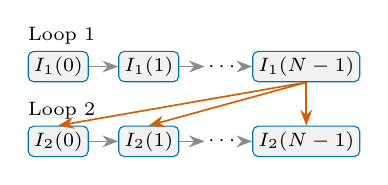
\begin{tikzpicture}[x=1cm,y=1cm,
 instance/.style={draw=origblue,rounded corners=2pt,fill=boxgray,inner sep=2pt,font=\scriptsize},
 carry/.style={->,draw=rulegray},
 dependency/.style={->,draw=staleorange,semithick}]
\node[instance] (a) at (0,0) {$I_1(0)$};
\node[instance] (b) at (1.15,0) {$I_1(1)$};
\node[font=\scriptsize,inner sep=1pt] (gap1) at (2.10,0) {$\cdots$};
\node[instance] (c) at (3.15,0) {$I_1(N-1)$};
\node[instance] (d) at (0,-0.95) {$I_2(0)$};
\node[instance] (e) at (1.15,-0.95) {$I_2(1)$};
\node[font=\scriptsize,inner sep=1pt] (gap2) at (2.10,-0.95) {$\cdots$};
\node[instance] (f) at (3.15,-0.95) {$I_2(N-1)$};
\node[font=\scriptsize,anchor=south west,inner sep=0pt]
  at ([yshift=2pt]a.north west) {Loop 1};
\node[font=\scriptsize,anchor=south west,inner sep=0pt]
  at ([yshift=2pt]d.north west) {Loop 2};
\foreach \s/\t in {a/b,b/gap1,gap1/c,d/e,e/gap2,gap2/f} \draw[carry] (\s) -- (\t);
\foreach \t in {d,e,f} \draw[dependency] (c.south) -- (\t.north);
\end{tikzpicture}
\caption{Schematic of dependent reductions.}
\label{fig:dependent-loops}
\vspace{-6pt}
\end{wrapfigure}

In a \emph{dependent reduction}, the reduction body uses a value determined by an earlier reduction's final result over the same axis.
Such a value is its \emph{context}: it is invariant along the reduction axis, but becomes available only after the earlier computation completes.
In \cref{fig:dependent-loops}, $I_i(j)$ denotes iteration $j$ of loop $i$, and the orange arrows show the dependency between the loops.

Fusing these reductions into a single pass therefore requires accumulating information for the later reduction before its final context is available.
An aggregate quantity retained for a part of the input is a \emph{state component}, or \emph{state}; the retained quantities form its \emph{state tuple}.

A \emph{join} combines the tuples of two disjoint parts into the tuple for their union.
For results computed with local contexts, this operation must account for the change from each part's context to that of the union.
The two connected questions are therefore which states retain enough information and how to derive a join that updates those states correctly.

Developing such algorithms requires specialised expertise.
Online normalisation, moment accumulation and tiled attention require identifying retained quantities, deriving updates, and implementing and tuning kernels~\citep{milakov,chan,pebay,flashattention}.
Recent automatic fusion methods handle algebraic corrections such as shifting or rescaling partial results~\citep{neptune,redfuser}.
Their correction rules do not cover dependencies that require aggregate information beyond the existing reduction results.

\textbf{Our Work.}
We present \sys,\footnote{Greek \emph{hapax}, ``once''.} which fuses dependent tensor reductions by augmenting source reduction results and deriving their joins.
We draw on methods developed for divide-and-conquer parallelisation: Farzan and Nicolet synthesise auxiliary accumulators and joins~\citep{farzan17,farzan21}, while AutoLifter synthesises auxiliary values and combinators for divide-and-conquer computations~\citep{autolifter}.
These methods introduce extra information so that results from independently processed parts can be combined.
\sys adapts this idea to fusion: \emph{auxiliary states} supplement source results with information needed for their context corrections.

\par\medskip
\noindent\begin{minipage}{\linewidth}
\begin{minipage}[t]{0.50\linewidth}
\vspace{0pt}
Each part computes its state tuple using its own contexts; a join corrects and combines these tuples (\cref{fig:dc-fusion}).
Although computing a larger part's tuple may take multiple traversals, a singleton tuple depends on just one input element.
In this formulation, a {\bfseries fused loop} can be viewed as sequentially joining singleton state tuples in one traversal.
\end{minipage}\hfill
% Shared English vector figure; both prose editions include this source.
% The introducing prose occupies the other half of the enclosing minipage.
\begin{paperdiagram}
\captionsetup{type=figure,skip=4pt}
\centering
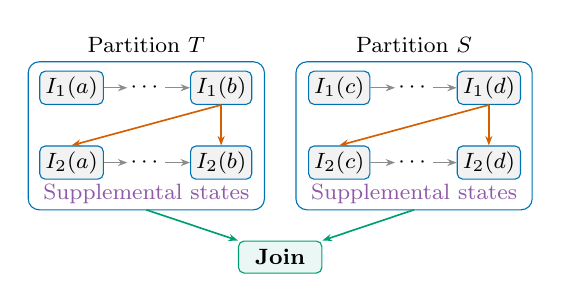
\begin{tikzpicture}[x=1cm,y=1cm,>={Stealth[length=1.2mm,width=0.9mm]},
  label/.style={font=\footnotesize,align=center},
  instance/.style={draw=origblue,rounded corners=2pt,fill=boxgray,
    inner sep=2pt,minimum height=0.32cm,font=\footnotesize},
  continuation/.style={font=\footnotesize,inner sep=1pt},
  part/.style={draw=origblue,rounded corners=4pt},
  joinop/.style={draw=fixgreen,rounded corners=2pt,fill=fixgreen!8,
    inner xsep=6pt,inner ysep=3pt,font=\footnotesize\bfseries},
  carry/.style={->,draw=rulegray},
  dependency/.style={->,draw=staleorange,semithick},
  combine/.style={->,draw=fixgreen,semithick}]

\node[label] at (1.50,0) {Partition $T$};
\node[label] at (4.90,0) {Partition $S$};
\draw[part] (0,-0.22) rectangle (3.00,-2.10);
\draw[part] (3.40,-0.22) rectangle (6.40,-2.10);

% Symbolic endpoints stand for the first and last iterations of each part.
\node[instance] (t1a) at (0.55,-0.55) {$I_1(a)$};
\node[continuation] (t1dots) at (1.50,-0.55) {$\cdots$};
\node[instance] (t1b) at (2.45,-0.55) {$I_1(b)$};
\node[instance] (t2a) at (0.55,-1.50) {$I_2(a)$};
\node[continuation] (t2dots) at (1.50,-1.50) {$\cdots$};
\node[instance] (t2b) at (2.45,-1.50) {$I_2(b)$};
\node[instance] (s1c) at (3.95,-0.55) {$I_1(c)$};
\node[continuation] (s1dots) at (4.90,-0.55) {$\cdots$};
\node[instance] (s1d) at (5.85,-0.55) {$I_1(d)$};
\node[instance] (s2c) at (3.95,-1.50) {$I_2(c)$};
\node[continuation] (s2dots) at (4.90,-1.50) {$\cdots$};
\node[instance] (s2d) at (5.85,-1.50) {$I_2(d)$};
\foreach \a/\dots/\b in {t1a/t1dots/t1b,t2a/t2dots/t2b,s1c/s1dots/s1d,s2c/s2dots/s2d} {
  \draw[carry] (\a.east) -- (\dots.west);
  \draw[carry] (\dots.east) -- (\b.west);
}
% Each part's completed first reduction supplies its second reduction.
\foreach \a/\b in {t1b/t2a,t1b/t2b,s1d/s2c,s1d/s2d}
  \draw[dependency] (\a.south) -- (\b.north);
\node[label,text=auxpurple] at (1.50,-1.90) {Supplemental states};
\node[label,text=auxpurple] at (4.90,-1.90) {Supplemental states};

\node[joinop] (combined) at (3.20,-2.70) {Join};
\draw[combine] (1.50,-2.10) -- (combined.north west);
\draw[combine] (4.90,-2.10) -- (combined.north east);
\end{tikzpicture}
\caption{Partitioned computation.}
\label{fig:dc-fusion}
\end{paperdiagram}

\end{minipage}\par\medskip

To determine what information can support such a join, \sys separates reduction bodies from their contexts algebraically.
The resulting \emph{reference states} are reductions whose bodies do not read those contexts, hence are \emph{context-independent}.
They combine independently and determine the required results, establishing a single-pass construction when the analysis succeeds.
Their number gives a sufficient state-count bound independent of the reduction length.

The reference construction provides a valid single-pass representation, but executing its expanded arithmetic may undo source centring or scaling and introduce cancellation or overflow~\citep{chan,blanchard,boldo_fp}.
These numerical concerns motivate starting the \emph{maintained state tuple}---the quantities accumulated by the fused program---from source reduction results computed in local contexts.
Retaining these results keeps the source's centred or scaled quantities available for context corrections.
When the source results do not contain enough information for these corrections, auxiliary states supply the missing information.

\sys synthesises auxiliary states that, together with the source reduction results, form a maintained tuple convertible to and from the reference tuple.
For each candidate tuple, the synthesis procedure constructs and verifies the conversion expressions.
These conversions yield a correct join by recovering the reference tuples of the input parts, applying their known join, and reconstructing the maintained tuple of the union.
Thus, synthesis searches for auxiliary states satisfying this conversion requirement, without separately searching for join expressions.

To constrain the auxiliary-state search space, we construct candidate expressions from how the source reduction results respond to context changes.
Symbolically shifting or scaling a local context exposes aggregate coefficients needed to correct its result.
These coefficients provide candidate expressions for syntax-guided synthesis, restricting the search to quantities with a role in the update.
Together, fixed source components and these candidates limit what the synthesiser must invent.
The same corrections provide execution formulas that adjust local results while reusing source centring and scaling where possible.
Verifying these formulas against the join obtained through recovery connects the numerical formulation to the algebraic correctness argument.

Over the reals, the resulting join computes the maintained state tuple of the combined input.
Because the join also applies to arbitrary disjoint non-empty parts, the derived reducer admits independent computations on parts followed by a reduction tree.
Fewer traversals create opportunities for reducing data movement; realised performance also depends on state size, join cost and scheduling.

We implement \sys as a rewrite of TVM tensor expressions (TE)~\citep{tvm}.
A recorded implementation snapshot derives single-pass reducers for \nShowFused of \nShowcase selected operators from machine learning and scientific computing.
We report coverage, discovered states and derivation cost, and describe the implemented MPFR validation used to compare the emitted programs' accuracy with their sources.
GPU scheduling and performance evaluation remain subsequent work.

\noindent This paper makes the following contributions:
\begin{itemize}
\item \textbf{Fusion of dependent-reduction patterns.}
Context separation identifies a class of dependent chains with a single-pass construction, including consumer bodies outside the stated algebraic conditions of recent automatic fusion methods, and bounds the states sufficient for this construction.
\item \textbf{Reference-guided state synthesis and join derivation.}
Complete recovery of a reference representation reduces synthesis to state augmentation and makes a separate search for join expressions unnecessary.
\item \textbf{Source-guided search and numerical formulation.}
Source results and their context corrections restrict auxiliary-state search while providing execution formulas that reuse source centring and scaling where possible.
\item \textbf{Implementation and evaluation.}
A TVM implementation and recorded results on coverage, discovered states and derivation cost for \nShowcase operators.
\end{itemize}

% Allow the overview to float near the section opening without blocking prose.
% Shared English visual; both prose editions include this source.
\par\medskip
\noindent\begin{minipage}{\linewidth}
\captionsetup{type=figure}
\centering
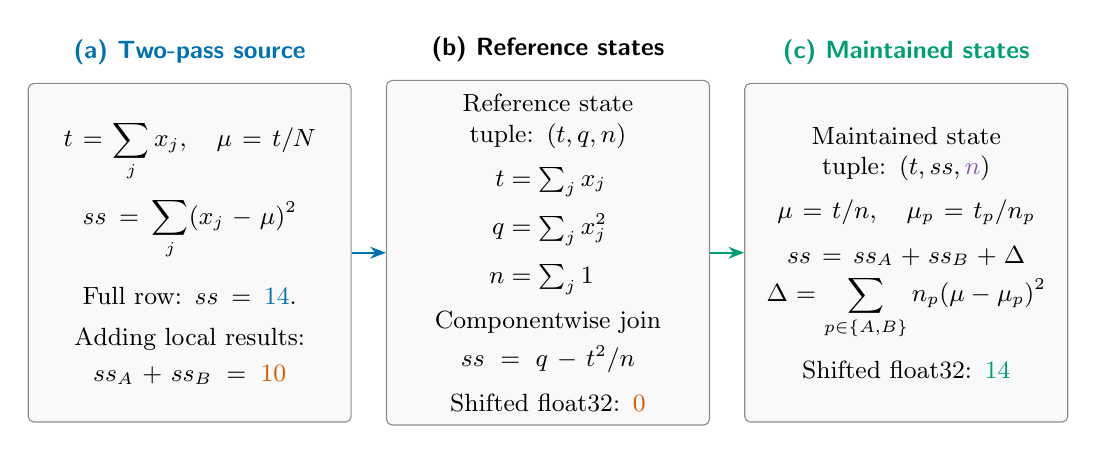
\begin{tikzpicture}[
  summary/.style={draw=rulegray,rounded corners=2pt,fill=boxgray!45,
    text width=3.75cm,minimum height=4.3cm,inner sep=5pt,
    align=center,font=\small},
  heading/.style={font=\sffamily\small\bfseries,anchor=south}]
\node[summary] (source) at (0,0) {
  $\displaystyle t=\sum_j x_j,\quad \mu=t/N$\\[5pt]
  $\displaystyle ss=\sum_j(x_j-\mu)^2$\\[9pt]
  Full row: $ss=\orig{\exTwoPass}$.\\[4pt]
  Adding local results:\\[2pt]
  $ss_\pa+ss_\pb=\stale{\exNaive}$
};
\node[summary] (reference) at (4.55,0) {
  Reference state tuple: $(t,q,n)$\\[5pt]
  $\begin{aligned}
    t&=\textstyle\sum_j x_j\\[2pt]
    q&=\textstyle\sum_j x_j^2\\[2pt]
    n&=\textstyle\sum_j 1
  \end{aligned}$\\[5pt]
  Componentwise join\\[3pt]
  $ss=q-t^2/n$\\[5pt]
  Shifted float32: $\stale{\exTextbookFloat}$
};
\node[summary] (maintained) at (9.1,0) {
  Maintained state tuple: $(t,ss,\aux{n})$\\[5pt]
  $\mu=t/n,\quad \mu_p=t_p/n_p$\\[5pt]
  $ss=ss_\pa+ss_\pb+\Delta$\\[3pt]
  $\displaystyle\Delta=\sum_{p\in\{\pa,\pb\}}n_p(\mu-\mu_p)^2$\\[7pt]
  Shifted float32: $\fix{\exTwoPassFloat}$
};
\node[heading,text=origblue] at ([yshift=3pt]source.north) {(a) Two-pass source};
\node[heading] at ([yshift=3pt]reference.north) {(b) Reference states};
\node[heading,text=fixgreen] at ([yshift=3pt]maintained.north) {(c) Maintained states};
\draw[flow] (source.east) -- (reference.west);
\draw[flow,draw=fixgreen] (reference.east) -- (maintained.west);
\end{tikzpicture}
\caption{Deriving a single-pass variance reducer.
For $\pa=(1,3)$ and $\pb=(2,6)$, adding locally centred results loses the change of mean.
The reference state tuple establishes a three-state bound; the maintained state tuple retains $t$ and $ss$ and adds \aux{$n$} for the correction.
The shifted results report $ss$ after adding $10^4$ to every input.}
\label{fig:variance}
% src: data/illus.json variance_exact and variance_float32
\end{minipage}\par\medskip

\begingroup
\setlength{\intextsep}{2pt}
\reservewrapspace{12\baselineskip}
\section{Motivating Example}
\label{sec:example}

\begin{wrapfigure}{r}{0.48\textwidth}
\begin{lstlisting}[style=pseudocode,caption={Two-pass source program.},label={lst:variance-before}]
Input: $x_0,\ldots,x_{N-1}$, $N>0$
$t\gets0$
for $j=0,\ldots,N-1$:
    $t\gets t+x_j$
$\mu\gets t/N$
$ss\gets0$
for $j=0,\ldots,N-1$:
    $ss\gets ss+(x_j-\mu)^2$
return $\;ss/N$
\end{lstlisting}
\end{wrapfigure}
Variance illustrates the dependency that fusion must remove.
For a row of length $N$, the source program in \cref{lst:variance-before} first computes the total $t$ and the mean $\mu=t/N$, then accumulates the centred sum of squares $ss$; the variance is $ss/N$.
The second traversal cannot begin its original computation until the first has produced the final mean.

To replace this dependency with a join, we first consider results computed using local means.
For a non-empty part $S$, let $t_S$ and $ss_S$ be its source reduction results and $\mu_S$ its mean.
Computing these results directly still takes two passes over that part.
For disjoint parts $\pa$ and $\pb$, applying the source reduction operator, $\oplus=+$ in this example, gives $ss_\pa\oplus ss_\pb=ss_\pa+ss_\pb$.
This does not generally equal the centred sum for their union: the two local results use different means, as \cref{fig:variance}(a) illustrates.
A correct join must account for the change to a common mean.

We therefore first seek states that can be combined without sharing a mean.
Expanding the centred reduction makes its dependence on $\mu_S$ explicit:
\begin{equation}
\label{eq:variance-reference}
ss_S=\sum_{j\in S}(x_j-\mu_S)^2
=\underbracket{\colorbox{boxgray}{$\displaystyle\sum_{j\in S}x_j^2$}}_{q_S}
 -2\mu_S\underbracket{\colorbox{boxgray}{$\displaystyle\sum_{j\in S}x_j$}}_{t_S}
 +\mu_S^2\underbracket{\colorbox{boxgray}{$\displaystyle\sum_{j\in S}1$}}_{n_S}.
\end{equation}
The highlighted reductions do not read $\mu_S$: they are the square sum $q_S$, the total $t_S$ and the count $n_S$.
They form the reference state tuple $(t_S,q_S,n_S)$ in panel (b).
Each state combines by addition, and together they recover the source result through $\mu_S=t_S/n_S$ and $ss_S=q_S-t_S^2/n_S$.
This establishes a sufficient three-state representation, independent of the input length.

The reference representation makes a single pass algebraically possible, but its reconstruction of $ss$ subtracts potentially large, nearly equal quantities.
The shifted float32 input in \cref{fig:variance} illustrates the resulting cancellation.
To retain the centred computation, \sys instead starts from the source results $(t,ss)$ and analyses what their correction requires.
Let $\mu$ be the mean of the union and $\delta_\pa=\mu-\mu_\pa$ its change on $\pa$.
Expanding around the local mean gives
\begin{equation}
\label{eq:variance-rebase}
\sum_{j\in\pa}(x_j-\mu)^2
=ss_\pa-2\delta_\pa\sum_{j\in\pa}(x_j-\mu_\pa)+\delta_\pa^2 n_\pa
=ss_\pa+\delta_\pa^2 n_\pa.
\end{equation}
The linear term vanishes because deviations from a partition's own mean sum to zero.
The remaining correction is weighted by $n_\pa$, the number of elements whose centre changes.
The source results $(t_\pa,ss_\pa)$ do not retain this count.
Thus context-correction analysis exposes $n$ as information missing from the chosen representation, and \sys tests it as an auxiliary state.
Here that coefficient alone supplies a sufficient augmentation: since $n_S>0$, the maintained state tuple $(t_S,ss_S,n_S)$ recovers $q_S=ss_S+t_S^2/n_S$, with the other reference states read directly.
The state-selection procedure verifies this recovery before accepting the tuple.

\reservewrapspace{14\baselineskip}
\begin{wrapfigure}{r}{0.48\textwidth}
\begin{lstlisting}[style=pseudocode,caption={Fused single-pass program.},label={lst:variance-after}]
$\leaf(x)=(x,0,1)$
function $\Mrg(\pa,\pb)$:
    $t\gets t_\pa+t_\pb$; $n\gets n_\pa+n_\pb$
    $\mu\gets t/n$; $ss\gets ss_\pa+ss_\pb$
    for $p\in\{\pa,\pb\}$:
        $ss\gets ss+n_p(\mu-t_p/n_p)^2$
    return $\;(t,ss,n)$
$(t,ss,n)\gets\leaf(x_0)$
for $j=1,\ldots,N-1$:
    $(t,ss,n)\gets\Mrg((t,ss,n),\leaf(x_j))$
return $\;ss/n$
\end{lstlisting}
\end{wrapfigure}
Using the recovery to derive a join and expressing it around the local means gives panel (c).
The join adds totals and counts, and corrects each local centred sum to the combined mean before adding them.
\sys verifies that the result is the maintained state tuple of the union.
On the illustrated shifted input, the corrected join matches the two-pass result.

To turn this join into fusion, choose each part to contain exactly one element.
Its mean is $x_j$, its centred sum is zero and its count is one, so its maintained state tuple is immediately $\leaf(x_j)=(x_j,0,1)$.
\Cref{lst:variance-after} initialises the running tuple from the first element and computes and joins each subsequent tuple as its element is read.
This removes the local traversals as well as the global dependency: the input is read once, and the final variance is $ss/n$.
Subscripts in the listing identify fields of the two input tuples.

Over the reals, the resulting join recovers the pairwise variance formula of \citet{chan} and, applied one element at a time, is algebraically equivalent to Welford's update~\citep{welford}.
The same union property also permits a parallel reduction tree.
\endgroup

\section{System Overview}
\label{sec:chains}

\subsection{Derivation Pipeline}

\sys takes a program expressed in TVM Tensor Expressions (TE) and the declared domain of its inputs.
As shown in \cref{fig:pipeline}, it first extracts dependent reduction chains over a shared axis (\cref{sec:input-chains}) and then derives a single-pass replacement for each chain.
For each extracted chain, algebraic analysis separates each reduction's context from its input-dependent terms.
The resulting reference states join independently and determine the outputs, establishing a sufficient single-pass construction and a default limit on the maintained state count (\cref{sec:existence}).

\reservewrapspace{26\baselineskip}
\begin{wrapfigure}[26]{r}{0.48\textwidth}
\centering
% Shared vector source for the paper and standalone diagram.
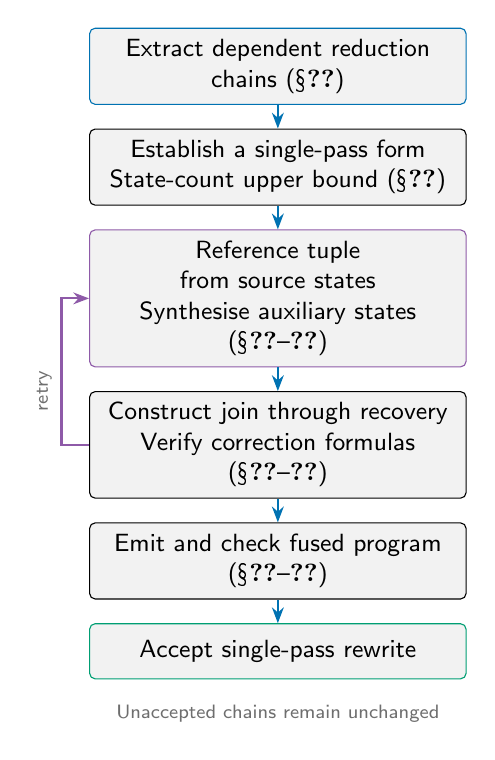
\begin{tikzpicture}[node distance=3mm,
  process/.style={stage,text width=4.5cm,font=\sffamily\small,minimum height=7mm}]
\node[process,draw=origblue] (extract) {Extract dependent reduction\\chains (\S\ref{sec:input-chains})};
\node[process,below=of extract] (judge) {Establish a single-pass form\\State-count upper bound (\S\ref{sec:existence})};
\node[process,below=of judge,draw=auxpurple] (candidate) {Reference tuple from source states\\Synthesise auxiliary states\\(\S\ref{sec:selection}--\ref{sec:synthesis})};
\node[process,below=of candidate] (derive) {Construct join through recovery\\Verify correction formulas\\(\S\ref{sec:recovery}--\ref{sec:rebase})};
\node[process,below=of derive] (check) {Emit and check fused program\\(\S\ref{sec:accuracy}--\ref{sec:impl})};
\node[process,below=of check,draw=fixgreen] (output) {Accept single-pass rewrite};
\foreach \a/\b in {extract/judge,judge/candidate,candidate/derive,derive/check,check/output}
  \draw[flow] (\a) -- (\b);
\draw[flow,draw=auxpurple] (derive.west) -- ++(-0.35,0) |- (candidate.west);
\node[lbl,rotate=90,anchor=south] at ([xshift=-3.5mm]derive.north west) {retry};
\node[lbl,below=2mm of output] {Unaccepted chains remain unchanged};
\end{tikzpicture}

\caption{End-to-end derivation.}
\label{fig:pipeline}
\end{wrapfigure}
Selection starts with the source reduction results as the initial maintained states.
For a source result that is undefined on a legal non-empty part, the procedure seeks a defined representation by extracting the offending context and retaining its coefficients.
Expanding the definitions of these initial states yields their reference tuple and the expressions reconstructing them from it.
This tuple fixes the information that auxiliary-state synthesis must retain.
To discover missing information, the analyser derives how each retained result changes when its local context is replaced by the context of a larger part.
The coefficients of these corrections provide candidate auxiliary states.
The procedure first checks the initial tuple alone, then this tuple augmented with all admissible correction coefficients.
Only if neither tuple succeeds within the state limit does syntax-guided synthesis search combinations of these candidate expressions and, subsequently, reference states.
The search therefore concerns only auxiliary states that, together with the source states, recover the reference tuple (\cref{sec:selection,sec:synthesis}).

For each proposed maintained tuple, verification constructs expressions recovering this entire reference tuple and proves their identities and definedness on legal parts.
This recovery defines a symbolic join: recover the reference states of the two parts, combine them independently, and express the result in maintained states.
Verification establishes that the joined tuple is the state tuple of the union; unsuccessful proofs return to state selection within the search limits.
For execution, context-correction analysis constructs formulas on the maintained states and their local contexts, and verifies them against this symbolic join.
These formulas reuse source centring and scaling where possible to retain its numerical structure; a component without such a formula uses the symbolic join expression (\crefrange{sec:recovery}{sec:rebase}).

The backend emits a TE program that initialises a singleton state tuple for each input element, joins the tuples, and reconstructs the outputs from the maintained states using the source program's scalar dependencies.
Static checks on the reducer and differential numerical measurements in the rebuilt program determine acceptance of this floating-point implementation (\cref{sec:accuracy,sec:impl}).
If no verified construction is found, or emission or numerical checks fail, the source chain is retained.


\subsection{Input Reduction Chains}
\label{sec:input-chains}

The extracted chains contain reductions and intervening computations over a shared axis.
\Cref{fig:grammar} gives the language of reduction bodies; the definitions below specify the dependencies within a chain and its meaning on an input part.

\begin{figure}[htbp]
\small
\begin{align*}
f \;::=\;& x \mid \ctx \mid c \mid N
 \mid f + f \mid f - f \mid f \times f \mid f \div f
 \mid \exp f \mid \log f \mid \sqrt{f} \mid f^{k} \mid |f| \mid \max(f,f) \mid \min(f,f)\\
m \;::=\;& \textstyle\bigoplus_{j} f \mid g(\ctx_1,\dots,\ctx_p)
\end{align*}
\caption{Reduction bodies $f$ and chain members $m$. $x$ ranges over the values a chain reads at position $j$ of the axis, $\ctx$ over earlier members, $c\in\R$ over constants, $k\in\mathbb{Z}$, $N$ is the extent of the axis, and $\oplus\in\{\Sigma,\max,\min\}$.}
\label{fig:grammar}
\end{figure}

\begin{definition}[Reduction chain]
\label{def:chain}
Fix an axis $\Ax=\{0,\dots,N-1\}$ and, for each position $j\in\Ax$, the tuple $x_j$ of values that the chain reads at $j$ from tensors outside it.
A \emph{reduction chain} is a sequence of members $m_1,\dots,m_n$ in producer order.
A member is either a \emph{reduction} $m=\bigoplus_{j\in\Ax} f_m(x_j,\ctx_m)$ with $\oplus\in\{\Sigma,\max,\min\}$, or a \emph{value} $m=g_m(\ctx_m)$.
The \emph{contexts} $\ctx_m$ are the final values of earlier reductions, or scalar computations derived from them, that $m$ reads at an index that does not involve $j$.
They are invariant along the axis, although computing them may require completing earlier reductions.
A chain is \emph{dependent} if some reduction reads a context.
\end{definition}

In the running variance example, the final sum reads the mean as a context.
\sys extracts chains from TE programs by treating reductions over the shared axis as chain members and inlining elementwise tensors read along $j$ into their bodies.
A reduction over another axis, such as $QK^\top$ in attention, stays outside the chain and supplies values $x_j$.

To speak about a part of the axis, we evaluate the chain on that part alone.

\begin{definition}[Semantics on an input part]
\label{def:partial}
For a non-empty $S\subseteq\Ax$, $m(S)$ is the value of member $m$ when every reduction is evaluated over $S$ only and every context is its own value on $S$.
The interpretation of extent reads is fixed for each chain before analysis: reads of $N$ denote $|S|$ when the extent represents the size of the current part, or retain the full-input value $N$ when it is a fixed program parameter.
Both interpretations agree on the full input.
The program computes $m(\Ax)$.
\end{definition}

The declared input domain constrains the element values.
A legal part is any non-empty part of an input satisfying these constraints.
An original member may be undefined on such a part even when the full-input output is defined; a maintained state must be defined on every legal part.
A single pass must produce $m(\Ax)$, wherever the source output is defined, from information gathered part by part.

\subsection{Single-Pass Reducer Contract}

The generated program must initialise a state tuple from each element, join these tuples without revisiting the input, and recover the required outputs.
The following contract states the relation that each join must preserve over the reals.

\begin{definition}[Single-pass reducer]
\label{def:reducer}
A \emph{state map} is a tuple $\st=(\st_1,\dots,\st_k)$ of functions of non-empty parts.
For fixed non-reduction indices, each function is scalar-valued, so $\st(S)$ is a state tuple with components $\st_i(S)$; its size $k$ is fixed for a given reducer, independently of the reduction length $N$.
A \emph{single-pass reducer} for a chain is a tuple $(\leaf,\Mrg,\epi)$ of an initialisation function $\leaf(x_j)=\st(\{j\})$, a binary join $\Mrg$ and an output function $\epi$ such that, for all disjoint non-empty parts $\pa$ and $\pb$,
\begin{equation}
\label{eq:invariant}
\Mrg(\st(\pa),\st(\pb))=\st(\pa\dunion\pb),\qquad
\epi(\st(\Ax))=\bigl(m(\Ax)\bigr)_{m\text{ required}}.
\end{equation}
The \emph{required} members are those the rest of the program reads.
\end{definition}

The initialisation function produces a singleton state tuple for each input element; the generated reduction starts from the first tuple and folds the remaining tuples.
No numerical state tuple represents an empty part: execution skips empty parts, and the input axis must be non-empty.
The join invariant of \cref{eq:invariant} connects the maintained state tuple to the original program.

\begin{lemma}[Laws from the invariant]
\label{lem:laws}
If the invariant holds, $\Mrg$ is commutative and associative when applied to state tuples of pairwise disjoint non-empty parts.
For every partition of $\Ax$ into non-empty parts and every binary join tree over them, joining the leaves yields $\st(\Ax)$.
The serial fold initialised from its first singleton state tuple has the same property.
\end{lemma}

\begin{proof}
$\Mrg(\st(\pa),\st(\pb))=\st(\pa\dunion\pb)=\st(\pb\dunion\pa)=\Mrg(\st(\pb),\st(\pa))$, and associativity follows in the same way from that of $\dunion$.
The rest is induction on the join tree and on the length of the fold.
\end{proof}

Each non-empty part can therefore compute its state tuple independently.
A tree of joins combines these tuples without another traversal of the parts.
This parallel structure follows from the invariant, independently of a particular schedule.

In the vocabulary of program calculation, $S\mapsto\st(S)$ is a homomorphism from finite non-empty bags under $\dunion$ to the state tuples under $\Mrg$: equivalently, a list homomorphism~\citep{bird87,gibbons96} invariant under permutation of its input.
In the vocabulary of databases, a chain with a context-independent reference construction is an \emph{algebraic} aggregate, computable from a fixed number of \emph{distributive} ones~\citep{datacube}.
Empty parts are handled by control flow, outside the algebraic join contract.

\paragraph{Problem.}
Given a dependent chain, establish a sufficient condition for a single-pass reducer, construct one, prove \cref{eq:invariant}, and accept it only if in floating point it introduces no additional non-finite result on the checked inputs and its measured error stays within the stated acceptance threshold relative to the source program.

\section{A Sufficient Condition for a Single Pass}
\label{sec:existence}

A link reads its context at every position $j$, but the context's final value is known only at the end of the axis.
A single pass exists when every link can be \emph{freed} of its contexts: rewritten as a function of the contexts and of reductions that read none.
This section gives the rules that free a link, the algorithm that applies them, and what follows from them.

\subsection{Freeing a Reduction from Its Contexts}
\label{sec:freeing}

Say that an operation $\varphi$ \emph{commutes} with a reduction $\oplus$ if $\varphi(a\oplus b)=\varphi(a)\oplus\varphi(b)$.
\Cref{tab:rules} lists the operations \sys pulls out of a reduction; each is an identity over $\R$ under its side condition and where all expressions are defined.
A sum distributes over addition and permits factors independent of $j$ to be extracted.
A maximum permits extraction of an added term, a factor proven non-negative, or a non-decreasing function.
An even power or an absolute value of a context-dependent term becomes the larger of two extremes.

\begin{table}[t]
\footnotesize
\caption{Operations that commute with a reduction over $j$; $a$, $c$ and $y$ do not depend on $j$. Each rule is an identity under its side condition, which \sys proves syntactically before applying it.}
\label{tab:rules}
\begin{tabular}{@{}llp{0.42\linewidth}@{}}
\toprule
\textbf{Reduction} & \textbf{Rewrite} & \textbf{Side condition}\\
\midrule
$\sum_j$ & $\sum_j (u_j+v_j)=\sum_j u_j+\sum_j v_j$ & none\\
$\sum_j$ & $\sum_j a\,u_j=a\sum_j u_j$, \ $\sum_j e^{u_j+y}=e^{y}\sum_j e^{u_j}$ & none\\
$\max_j$ & $\max_j (u_j+a)=\max_j u_j+a$ & none\\
$\max_j$ & $\max_j c\,u_j=c\max_j u_j$ & $c\ge 0$ proven\\
$\max_j$ & $\max_j h(u_j)=h(\max_j u_j)$ & $h$ non-decreasing on the relevant domain\\
$\max_j$ & $\max_j |u_j|^{2k}=\max(\max_j u_j,\ \max_j -u_j)^{2k}$ & integer $k\ge1$\\
$\min_j$ & dual to $\max_j$ & dual\\
\bottomrule
\end{tabular}
\end{table}

The separation below splits the body into $r$ contributions.
Each $g_k$ contains the data-dependent part, while $\varphi_{k,\ctx}$ carries its dependence on the context.
The context is held fixed during regrouping; the resulting summaries can therefore be accumulated before its value is known.

\begin{lemma}[Regrouping]
\label{lem:regroup}
Let $f(x,\ctx)=\bigoplus_{k=1}^{r}\varphi_{k,\ctx}(g_k(x))$, where no $g_k$ reads a context and every $\varphi_{k,\ctx}$ commutes with $\oplus$.
Then for every non-empty part $S$, $\bigoplus_{j\in S} f(x_j,\ctx)=\bigoplus_{k=1}^{r}\varphi_{k,\ctx}\bigl(\bigoplus_{j\in S} g_k(x_j)\bigr)$.
\end{lemma}

\begin{proof}
Reorder the reduction by the associativity and commutativity of $\oplus$, then pull each $\varphi_{k,\ctx}$ out.
\end{proof}

The resulting tuple can be computed without knowing the final contexts. Those contexts are used only when reconstructing the required members from the tuple.

\subsection{The Judgement}
\label{sec:judge}

A reference atom is a context-free reduction $q(S)=\bigoplus_{j\in S}g(x_j)$, identified by its reduction operation and canonical body.
Constant bodies are allowed: $|S|=\sum_{j\in S}1$ is the atom with addition and body $1$.
Before collecting atoms, every read of the reduction-axis extent as a value is normalised to this sum under the partial semantics.
Extracting a constant term from a sum can expose the same atom.
Both occurrences enter the same collection and are shared by canonical equality; no atom is added unless a required expression uses it.

\begingroup
\setlength{\intextsep}{2pt}
\reservewrapspace{16\baselineskip}
\begin{wrapfigure}{r}{0.48\textwidth}
\begin{minipage}{\linewidth}
\begin{algorithm}[H]
\small
\caption{\textsc{Judge}$(\mathit{chain}, \mathit{req})$}
\label{alg:judge}
\KwOut{reference atoms $\mathcal Q$, or failure}
Normalise extent reads in $\mathit{chain}$\;
$W\leftarrow \mathit{req}$;\ $\mathcal Q\leftarrow\emptyset$\;
\While{$W$ not empty}{
  $m\leftarrow$ pop $W$\;
  $e\leftarrow$ free contexts from body of $m$\;
  push unvisited dependencies of $e$ onto $W$\;
  \ForEach{atom $q$ in $e$}{
    \lIf{$q$ reads a context}{\Return \textsc{Stuck}$(m,q)$}
    $\mathcal Q\leftarrow\mathcal Q\cup\{q\}$ (canonical form)\;
  }
}
\Return \textsc{Fusible}$(\mathcal Q)$\;
\end{algorithm}
\end{minipage}
\end{wrapfigure}
\Cref{alg:judge} visits every required member and its dependencies, processing each member once.
It replaces each context by a symbol constant along the axis, rewrites the body with \cref{tab:rules}, and collects the remaining atoms in $\mathcal Q$.
An atom that still reads a context is \emph{stuck}: the rules could not free it.
Otherwise the collected atoms constitute the reference state tuple, with one state per distinct atom.

The construction gives a finite summary whose components join independently and whose values determine the required outputs.
Its size bounds the number of states in this construction; selection uses that bound as its default state limit.
It also identifies the context-free quantities against which a selected representation can be verified.
These roles are distinct: the existence of this construction does not establish that every representation preserving the original results fits the same limit.

\finishwrapspace
\endgroup

\begin{theorem}[Existence]
\label{thm:existence}
Suppose \textsc{Judge} returns \textsc{Fusible}$(\mathcal Q)$, with
\[
\mathcal Q=\{q_1,\dots,q_k\},\qquad
q_i(S)=\bigoplus_{j\in S}^{(i)}g_i(x_j).
\]
If the collected bodies are defined on the declared element domain, the chain has a single-pass reducer with at most $|\mathcal Q|$ states.
Its state tuple is $(q_1(S),\dots,q_k(S))$, its join is componentwise, and its epilogue reconstructs the required outputs on their source domain.
\end{theorem}

\begin{proof}[Proof sketch]
Extent normalisation preserves partial semantics, and every algebraic rewrite is an identity over $\R$ on its source domain under its proven side condition.
By \cref{lem:regroup} and induction over producer order, each required member has a reconstruction expression in the collected atoms wherever the source computation is defined.
For every atom, $q_i(S\dunion T)=q_i(S)\oplus_i q_i(T)$.
The tuple therefore joins componentwise and has leaf $(g_1(x_j),\dots,g_k(x_j))$.
The domain assumption makes these states defined on legal non-empty partitions; applying the reconstruction expression at the root gives the required outputs.
There is one coordinate per atom, establishing the bound.
\end{proof}

The judgement recognises chains whose contexts can be separated by these rules.
When a residual reduction still depends on a context, the analysis stops without producing a construction.
Further identities or stronger input relations may establish reducibility beyond this recognised class.

The construction is an algebraic reference, not necessarily the numerical form we should execute.
Separating contexts from reduction bodies changes the intermediate quantities: cancelling terms may become large independent sums, and bounded expressions may become products of unbounded factors.
Keeping the source reduction results preserves their centring and scaling, while auxiliary states provide the information needed for a join.
The next step is therefore to derive a maintained representation and prove that it retains the required information of the construction.

\section{Synthesising States and Deriving the Reducer}
\label{sec:derivation}

The source reduction results provide the starting point for our maintained representation.
Expanding their definitions into context-independent reductions gives a reference state tuple whose components already have joins.
We use this tuple to specify the information that auxiliary states must supply: together with the retained source states, they must recover every reference component.
Synthesis therefore searches only for auxiliary states.
Once a recovery map is constructed and verified, the join follows by composition.
This section develops that process through a Householder-type norm, where the implementation uses synthesis to select an auxiliary state.

\subsection{Source States and Reference Representation}
\label{sec:selection}

Let $\stsrc(S)$ denote the source-derived initial state tuple on a legal non-empty part $S$.
These states retain the source definitions whenever they are defined on legal parts.
A demonstrated domain defect is repaired by extracting the offending context: its coefficients replace that reduction in $\stsrc$, and the source result is reconstructed for the outputs.
We then expand these definitions using the context-separation rules, substitute the definitions of their contexts, and collect the distinct context-independent reductions.
Their values form the reference tuple $\stref(S)$, and the expanded expressions give a known map $\Gsrc$:
\begin{equation}
\label{eq:source-reference}
\stsrc(S)=\Gsrc(\stref(S)).
\end{equation}
The reference components join independently and remain fixed throughout auxiliary-state search.
Whereas the existence analysis starts from the required outputs, this construction starts from the source states that the fused program will retain.

For the running example, consider two input sequences $x_j,e_j$.
A Householder-type norm first computes a squared norm $q_S$ and then uses $k_S=\sqrt{q_S}$ as the context of a second reduction:
\[
q_S=\sum_{j\in S}x_j^2,\qquad
v_S=\sum_{j\in S}(x_j+k_Se_j)^2.
\]
Thus $\stsrc(S)=(q_S,v_S)$; the scalar computation $k_S$ adds no reduction state.
Expanding the second definition exposes two further context-independent quantities,
\[
u_S=\sum_{j\in S}e_j^2,\qquad
p_S=\sum_{j\in S}x_je_j,\qquad
v_S=q_S+2k_Sp_S+q_Su_S.
\]
We obtain $\stref(S)=(q_S,u_S,p_S)$ and
$\Gsrc(q,u,p)=(q,q+2\sqrt q\,p+qu)$.
The two source states leave the information in $u$ and $p$ combined; auxiliary-state synthesis determines what additional information to retain.

\subsection{Discovering and Synthesising Auxiliary States}
\label{sec:synthesis}

Candidate expressions come from how a retained result changes with its context.
The analyser symbolically shifts or scales the local contexts and separates the resulting terms.
For a sum state $r$, a successful decomposition under the algebraic rules has the form
\begin{equation}
\label{eq:features}
r(S;\kappa')=\sum_{\ell}\alpha_\ell(\delta,\rho)\,e_\ell(S;\kappa_S),
\end{equation}
where $\kappa_S$ is the local context, $\kappa'$ the target context, and $\delta,\rho$ describe their additive or multiplicative changes.
The factors $\alpha_\ell$ depend on these changes; the aggregate coefficients $e_\ell$ expose information needed to correct the retained result.
Terms with different correction factors can also provide separate candidates.
For extrema, the corresponding monotonicity and context-extraction rules serve this role.
Each candidate has a definition in $\stref$ for reasoning and a structural reduction expression retaining local contexts for code generation.
The retained candidates form $\mathcal T_{\mathrm{pre}}$; each is a defined function of the reference tuple and fixed program parameters.

In the Householder example, writing $v_S(k)=\sum_{j\in S}(x_j+ke_j)^2$ gives
\[
v_S(k_S+\delta)
 =v_S+2\delta(p_S+k_Su_S)+\delta^2u_S.
\]
Besides the retained $v_S$, this correction exposes $p_S+k_Su_S$ and $u_S$.
Adding both gives four maintained states, while the existence construction supplies a default limit of three.
The search must therefore select a smaller augmentation.

Let $C=(c_1,\ldots,c_w)$ be the auxiliary expressions to be synthesised.
For a reference value $\xi$, their definitions determine
\[
G(\xi)=(\Gsrc(\xi),C(\xi)),\qquad
\st(S)=G(\stref(S)).
\]
We require $\st$ to recover $\stref$, a sufficient condition for constructing a join for the entire maintained tuple.
The synthesis specification expresses this information requirement before recovery is constructed.
Let $\mathcal R$ conservatively contain all reachable reference tuples, constrained by finite-sum facts and proved definedness conditions for $\Gsrc$ and the candidates.
For fixed program parameters, synthesis requires
\begin{equation}
\label{eq:synthesis}
\forall \xi,\eta\in\mathcal R:\quad
\bigl(\Gsrc(\xi)=\Gsrc(\eta)\ \land\ C(\xi)=C(\eta)\bigr)
\ \Longrightarrow\ \xi=\eta.
\end{equation}
Auxiliary states must distinguish reference tuples that the initial states cannot distinguish.
The known reference join then supplies the basis for joining the selected representation, so no join expression is included among the synthesis unknowns.

The candidate expressions in a set $\mathcal T$ serve as grammar terminals. Each auxiliary expression is drawn from the finite grammar
\[
\begin{aligned}
\mathcal E_1&::=e\quad(e\in\mathcal T),\\
\mathcal E_\ell&::=\mathcal E_{\ell-1}
 \mid\mathcal E_{\ell-1}+\mathcal E_1
 \mid\mathcal E_{\ell-1}-\mathcal E_1
 \qquad(2\le\ell\le d).
\end{aligned}
\]
\begingroup
\setlength{\intextsep}{4pt}
\reservewrapspace{21\baselineskip}
\begin{wrapfigure}{r}{0.48\textwidth}
\begin{minipage}{\linewidth}
\begin{algorithm}[H]
\small
\SetInd{0.5em}{0.7em}
\caption{\textsc{Select}$(\mathit{chain},b_{\max})$}
\label{alg:select}
$\stsrc\leftarrow$ source states after domain repair\;
$(\stref,\Gsrc)\leftarrow$ expand definitions of $\stsrc$\;
\lIf{preparation fails}{\Return keep source chain}
$\mathcal T_{\mathrm{pre}},K\leftarrow$ correction candidates\;
\ForEach{$M\in[\stsrc,(\stsrc,K)]$ fitting $b_{\max}$}{
\lIf{\textsc{Verify}$(M,\stref)$ succeeds}{\Return reducer}
}
\ForEach{$\mathcal T\in[\mathcal T_{\mathrm{pre}},\mathcal T_{\mathrm{mix}}]$}{
\ForEach{admissible auxiliary width $w$}{
\While{proposals and resources remain}{
Propose $C\in\mathcal E_d^{\,w}$\;
\lIf{\textsc{Verify}$((\stsrc,C),\stref)$ succeeds}{\Return reducer}
}
}}
\Return keep source chain\;
\end{algorithm}
\end{minipage}
\end{wrapfigure}
With the default $d=3$, expressions combine at most three occurrences of candidate terms.
A term can already be nonlinear in the reference values, so the grammar combines quantities discovered by analysis while preserving their structural forms.
The first grammar uses $\mathcal T_{\mathrm{pre}}$; the second also includes the reference components as candidate expressions.
When the existence analysis returns $\mathcal Q$, its bound $|\mathcal Q|$ supplies the default maintained-state limit $b_{\max}$.
The supplementary material establishes a general sufficient augmentation; the search here seeks a compact representation within this limit.

\Cref{alg:select} first tests $\stsrc$ alone, then its augmentation with the tuple $K$ of admissible correction coefficients.
It invokes synthesis if these choices do not yield a verified reducer within the state limit.
Here $\mathcal T_{\mathrm{mix}}$ contains $\mathcal T_{\mathrm{pre}}$ and the reference components; the auxiliary width satisfies $1\le w\le b_{\max}-|\stsrc|$.
For each proposal, \textsc{Verify} constructs recovery expressions, proves their identities and domains, and derives and verifies the complete reducer.
Search scheduling and solver limits are described with the implementation.

In the recorded Householder derivation, the initial tuple does not suffice and the complete coefficient augmentation exceeds the three-state limit.
SyGuS selects $C(q,u,p)=u$, giving $\st=(q,v,u)$.
The alternative coefficient $p+ku$ loses $u$ when $q=0$: then $p=k=v=0$ while $u$ can vary.
A later join can make the norm context non-zero, so these parts require different corrections.
The information requirement distinguishes these choices.
Selecting $u$ leaves only $p$ to be recovered, including at zero norm.
\finishwrapspace
\endgroup

\subsection{Constructing and Verifying Recovery}
\label{sec:atoms}
\label{sec:recovery}

For a proposed maintained tuple, the selected definitions give the known map $G$.
Recovery constructs an executable map $H$ from the equations defining that tuple, with
\begin{equation}
\label{eq:recovery}
H(G(\stref(S)))=\stref(S).
\end{equation}
The procedure substitutes known expressions and isolates unresolved reference components using supported algebraic rules.
Repeated substitution expresses every component in maintained states and fixed parameters.
Symbolic normalisation and SymPy establish identities, while Z3 proves domains and guarded implications.
This construction of $H$ is separate from the synthesis of $C$.

For Householder, $q$ and $u$ are retained directly.
Solving the definition of $v$ gives the remaining component and hence recovery:
\[
p=
\begin{cases}
0,&q=0,\\[2pt]
\dfrac{v-q-qu}{2\sqrt q},&q>0,
\end{cases}
\qquad H(q,v,u)=(q,u,p).
\]
\reservewrapspace{16\baselineskip}
% Both panels and their common caption form one full-width figure.
% Shared unchanged by the English and Chinese prose editions.
\par\medskip
\noindent\begin{minipage}{\linewidth}
\captionsetup{type=figure}
\centering
\begin{minipage}[t]{0.48\linewidth}
\vspace{0pt}
\centering
{\small\sffamily\bfseries (a) State relations}\par\medskip
% Shared vector source for the English and Chinese prose editions.
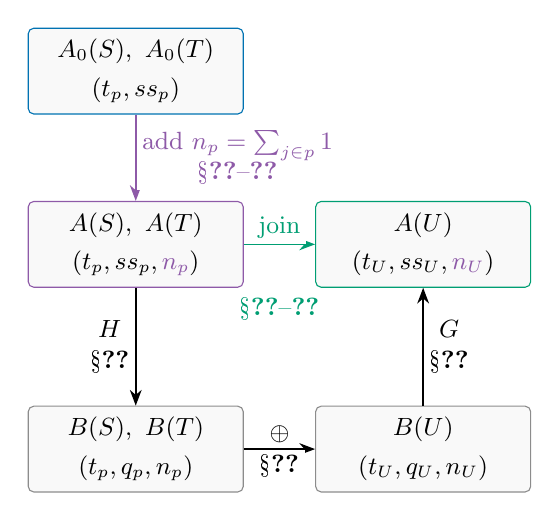
\begin{tikzpicture}[
  summary/.style={draw=rulegray,rounded corners=2pt,fill=boxgray!45,
    text width=2.45cm,minimum height=1.05cm,inner sep=4pt,
    align=center,font=\small},
  arrow/.style={-{Stealth[length=2mm]},semithick},
  label/.style={font=\small,fill=white,inner sep=2pt,align=center}]
\node[summary,draw=origblue] (original) at (0,2.2)
  {$A_0(S),\ A_0(T)$\\[3pt]$(t_p,ss_p)$};
\node[summary,draw=auxpurple] (maintained) at (0,0)
  {$A(S),\ A(T)$\\[3pt]$(t_p,ss_p,\aux{n_p})$};
\node[summary,draw=fixgreen] (merged) at (3.65,0)
  {$A(U)$\\[3pt]$(t_U,ss_U,\aux{n_U})$};
\node[summary] (reference) at (0,-2.6)
  {$B(S),\ B(T)$\\[3pt]$(t_p,q_p,n_p)$};
\node[summary] (combined) at (3.65,-2.6)
  {$B(U)$\\[3pt]$(t_U,q_U,n_U)$};
\draw[arrow,draw=auxpurple] (original) --
  node[label,right,text=auxpurple] {add $n_p=\sum_{j\in p}1$\\\S\ref{sec:selection}--\ref{sec:synthesis}} (maintained);
\draw[arrow,draw=fixgreen] (maintained) --
  node[label,above,text=fixgreen] {$\Mrg$}
  node[label,below=6mm,text=fixgreen] {\S\ref{sec:correctness}--\ref{sec:rebase}} (merged);
\draw[arrow] (maintained) -- node[label,left] {$H$\\\S\ref{sec:recovery}} (reference);
\draw[arrow] (reference) -- node[label,above] {$\oplus$}
  node[label,below] {\S\ref{sec:correctness}} (combined);
\draw[arrow] (combined) -- node[label,right] {$G$\\\S\ref{sec:atoms}} (merged);
\end{tikzpicture}

\end{minipage}\hfill
\begin{minipage}[t]{0.48\linewidth}
\vspace{0pt}
\small
\centerline{\sffamily\bfseries (b) Derivation}
\medskip
On each part, let $t=\sum_jx_j$, $q=\sum_jx_j^2$ and $n=\sum_j1$.
Expanding the source definition gives
\[
G(t,q,n)=(t,q-t^2/n,n).
\]
From $(t,ss)$, recovery leaves $q=ss+t^2/n$ dependent on the unknown $n$.
Adding $n$ gives the complete recovery
\[
H(t,ss,n)=(t,ss+t^2/n,n).
\]
Since $n>0$, both maps are defined and $H\circ G=\mathrm{id}$.
The reference join $\oplus$ adds coordinates.
The upper arrow follows by composition:
\[
\Mrg(a,b)=G\bigl(H(a)\oplus H(b)\bigr).
\]
With $t_U=t_S+t_T$ and $n_U=n_S+n_T$, rewriting yields the centred form
\[
\begin{aligned}
ss_U={}&ss_S+ss_T\\
&+\frac{n_Sn_T}{n_U}
  \left(\frac{t_S}{n_S}-\frac{t_T}{n_T}\right)^2.
\end{aligned}
\]
The emitted join evaluates this correction without materialising $q$.
\end{minipage}
\caption{Variance: auxiliary states, recovery and join derivation.
Here $p\in\{S,T\}$ and $U=S\dunion T$ for disjoint non-empty parts.
Arrow annotations identify the subsections that develop each step:
feature construction and synthesis (\S\ref{sec:selection}--\ref{sec:synthesis}), information equivalence (\S\ref{sec:recovery}),
join derivation (\S\ref{sec:correctness}), and numerical formulation (\S\ref{sec:rebase}).}
\label{fig:recovery-square}
\end{minipage}\par\medskip

The zero branch follows from $q=\sum_jx_j^2=0$: each $x_j$ is zero, so $p=\sum_jx_je_j=0$.
This is an instance of a finite-sum rule used by the verifier: a zero sum of non-negative terms forces each term to vanish.
Both branches recover the reference value on their domains, and a lazy conditional evaluates only the selected branch.
The resulting identity $H\circ G=\mathrm{id}$ establishes complete recovery, including legal zero-norm parts.

\Cref{fig:recovery-square} illustrates the construction: recover each part's $(q,u,p)$, add components, and apply $G$ to obtain the maintained tuple of the union.
Initialisation evaluates the state definitions on a singleton.
\finishwrapspace

\subsection{Deriving the Join and Proving Correctness}
\label{sec:correctness}

The reference components combine independently under $\oplus$, giving
$\stref(S\dunion T)=\stref(S)\oplus\stref(T)$ for disjoint non-empty parts.
Recovery therefore yields the maintained join by composition:
\begin{equation}
\label{eq:merge}
\Mrg(a,b)=G\bigl(H(a)\oplus H(b)\bigr).
\end{equation}

The output function $\epi$ follows the source program's scalar dependencies expressed in selected states; a retained output such as $v$ reads its own component.
Verification checks this reconstruction's identity and domain.

\begin{theorem}[Correctness over $\R$]
\label{thm:correct}
Let $\stref$ be defined on legal non-empty parts and join componentwise, and let $\st=G\circ\stref$.
Suppose $G$ and $H$ are defined on their reachable arguments and $H\circ G$ is the identity on reachable reference tuples.
If $\epi$ reconstructs the source outputs from $\st(\Ax)$ on their source domain, the derived reducer computes these outputs for any partition into non-empty parts and any binary join tree over them.
\end{theorem}
\begin{proof}
For disjoint non-empty parts,
\[
\begin{aligned}
\Mrg(\st(S),\st(T))
 &=G\bigl(H(G(\stref(S)))\oplus H(G(\stref(T)))\bigr)\\
 &=G\bigl(\stref(S)\oplus\stref(T)\bigr)\\
 &=G(\stref(S\dunion T))=\st(S\dunion T).
\end{aligned}
\]
Recovery gives the second equality and componentwise aggregation the third.
Initialisation supplies the singleton states, so induction over the tree yields $\st(\Ax)$ at the root.
Applying the verified output reconstruction completes the proof.
\end{proof}

This invariant covers every maintained component, including the auxiliary states.
The associativity and commutativity established in the reducer contract therefore apply to the derived join.
Complete reference recovery provides one common condition for selecting states and constructing their join.

\subsection{Numerical Formulation of the Join}
\label{sec:rebase}

The compositional join specifies the result to compute.
Its direct evaluation can reconstruct expanded reference quantities before recomputing maintained values; such intermediate subproblems can amplify error even when the overall computation is well conditioned~\citep{higham_decomposition}.
For execution, the context-change decompositions used in candidate discovery instead give formulas that correct the retained partial results to the joined context.
Recovery expresses the required coefficients in maintained states, and the corrected results combine under the source reduction operator.

For Householder, let $U=S\dunion T$, $k_P=\sqrt{q_P}$ and $\delta_P=k_U-k_P$ for $P\in\{S,T\}$.
The join adds $q$ and $u$ componentwise and updates the retained $v$ by
\[
v_U=\sum_{P\in\{S,T\}}
 \left[v_P+2\delta_P(p_P+k_Pu_P)+\delta_P^2u_P\right],
\]
where $p_P$ is recovered by the guarded expression above.
The formula retains each part's computed $v_P$ and adjusts it for the changed context.
Centred-moment joins and online softmax similarly correct partial results by recentring or rescaling~\citep{pebay,milakov}.

The verifier proves equality with \eqref{eq:merge} and definedness of the executed branches.
Components without a supported correction use their compositional expressions.
\begin{theorem}[Correctness of the emitted join]
\label{thm:printed}
An emitted join verified equal to the compositional join on reachable states, with its executed branches defined, satisfies the same join invariant.
\end{theorem}
\begin{proof}
Substitution of the verified equality preserves the invariant proved above.
\end{proof}
The emitted program then undergoes the static and differential numerical checks that determine floating-point acceptance.

\section{Keeping the Accuracy of the Original Program}
\label{sec:accuracy}

The derived reducer now has a verified join and a chosen numerical formulation.
It runs in floating point, where its evaluation order and intermediate values differ from those of the source~\citep{higham,goldberg}.
To decide whether this formulation is acceptable, \sys combines static checks on the emitted expressions with differential measurements against the original program.
The measurements use the following acceptance criterion.

\begin{definition}[Accuracy acceptance]
\label{def:gate}
Let the error of a result $\hat y$ be $\max|\hat y-y|/\max|y|$ against the reference result $y$, the original program evaluated in float64, and $\infty$ if any value of $\hat y$ is not finite.
A fused program \emph{passes the accuracy check} on a set of inputs if, on each of them, it produces a non-finite value only where the original does, and its error is at most $100\max(\mathit{err}_{\mathrm{orig}},\mathit{err}_{\mathrm{inh}})+64u$, where $\mathit{err}_{\mathrm{inh}}$ is an empirical sensitivity estimate from input perturbations and $u=2^{-23}$.
\end{definition}

The bound is relative to the original program, not to an exact answer: the fused program may lose what the original or the problem's conditioning already lose, up to a constant factor.
The check is applied to sampled inputs, so it is evidence, not a guarantee.

\subsection{Static Checks on the Emitted Join}
\label{sec:hazards}
\label{sec:static}

A single pass changes both the order of evaluation and the intermediate quantities.
Reassociation is inherent in parallel reductions, while expansion into raw moments can introduce cancellation and removal of scaling can expose overflow.
A further risk is division by a context that vanishes on a proper part even though it is non-zero on the full input.
These risks motivate retaining the source program's centring and scaling when the join admits that representation.

\textbf{Proven guarantees.}
\sys then checks two properties of the derived join.
Each is required of a candidate only if the original program has it.

\begin{proposition}[Bounded exponents]
\label{prop:exp}
Every argument of $\exp$ in the join is at most 8: each positive term is absorbed by a subtracted maximum over its own axis or by a running-maximum state.
\end{proposition}

\begin{proposition}[Positive divisors]
\label{prop:div}
Every executed divisor and logarithm argument checked by this condition is positive along the serial fold initialised from its first leaf.
The analysis combines a greatest fixpoint over the sign lattice $\{\text{any},\geq0,>0\}$ with SMT implications under branch guards.
\end{proposition}

\textbf{Where the join departs from the program.}
The program's own computation cannot always be kept.
When a source result is proved undefined on a legal partition, \textsc{Select} repairs its definition by moving the offending context outside the reduction and retaining the resulting coefficients as states.
% src: data/fused_ops.json actions; reducer/states.py and reducer/smt.py
A join that only re-bases the program's states is still an update formula, and on data whose offset is large relative to its spread an update formula can lose more than two passes do, by a factor of the problem's condition number~\citep{chan}.
In these cases nothing is proven about rounding error, and only the acceptance check below decides.

\subsection{Acceptance Measurements and Their Limits}
Rounding error is not decided by these proofs.
\sys therefore compares each fused program with the original before it accepts the fusion.
It evaluates both on inputs drawn from five families, centred, shifted by $10^4$, wide, and near the overflow and underflow thresholds, against a float64 interpretation of the original, and checks \cref{def:gate} on each family.
The families and the measurement are detailed in Appendix~E of the supplementary material.


\label{sec:accuracy-limits}

\Cref{tab:assurance} separates what \sys proves from what it checks on samples.
The acceptance check is a differential test on five families, not a proof: inputs it does not sample, such as exactly zero weights outside a declared positive domain, are not covered.
The execution contract excludes empty partitions from the join.
A parallel implementation must initialise each active partition from its own first leaf and skip inactive partitions, rather than inject a numerical identity.
This is a requirement on lowering, not a floating-point property established by the accuracy check.

\begin{table}[t]
\caption{What each step establishes. \tagP: proven; \tagS: checked on samples; ---: not established.}
\label{tab:assurance}
\footnotesize
\begin{tabular}{@{}lp{0.62\linewidth}l@{}}
\toprule
\textbf{Step} & \textbf{Property} & \\
\midrule
Judgement (\cref{alg:judge}) & defined reference atoms give a single pass with at most $|\mathcal Q|$ states & \tagP\\
Selection (\cref{alg:select}) & complete recovery and defined states on legal non-empty parts & \tagP\\
Join & invariant and leaves (\cref{thm:correct,thm:printed}) & \tagP\\
Join & bounded exponents, positive divisors on the serial fold (\cref{prop:exp,prop:div}) & \tagP\\
Rebuilt program & agrees with the original in float64 on three small shapes & \tagS\\
Rebuilt program & passes the accuracy check (\cref{def:gate}) on five input families & \tagS\\
Rebuilt program & a bound on its floating-point error for every input & ---\\
\bottomrule
\end{tabular}
\end{table}

\section{Implementation}
\label{sec:impl}

\sys is a Python package on top of TVM's tensor expressions, about \nLoC{} non-blank lines.
% src: gen/stats.tex nLoC (counted by scripts/gen_tex.py)
Its entry point \code{fuse(outputs, inputs)} rewrites every chain behind the outputs and returns the rewritten TE together with one report per chain; \code{judge(outputs)} runs only the reference-state construction.
The frontend reads chains from TE and translates reduction bodies into a symbolic form whose terms are hash-consed and kept canonical by the rewrites of \cref{tab:rules}.
Reference-state construction, state selection, join derivation and the proofs work on that form; SymPy handles identities not settled by canonical normalisation.
Internally, domain cardinality has a compact node representing the constant-body sum; the implementation reports it through a separate flag, equivalent to including that reduction in the reference set.
The frontend treats the full-input extent as a fixed parameter if it appears inside a reduction body other than as the divisor of the entire body; otherwise, extent reads denote the part's size.
This choice applies to the whole chain.
Z3 checks source domains, guarded recovery domains and injectivity of polynomial state representations over an abstraction of reachable states.
An unknown solver result rejects the obligation; it is never treated as a proof or as permission to replace a defined source result.
The back end emits each join as TE expressions and creates one \commreducer per chain, initialised from the first element's state tuple and joining the remaining elements' tuples.
It implements the output function as elementwise computations and rebuilds downstream tensors to read the new states.
A chain that is not fused is left exactly as written, and its report gives the reason.


Native cvc5 SyGuS~\citep{cvc5} searches for auxiliary states; it owns candidate enumeration and internal refinement.
Within each grammar stage, the implementation first tries the largest permitted number of auxiliary states, then smaller numbers in increasing order.
It allows at most 256 proposals, three occurrences of candidate expressions per auxiliary state and a 20-second synthesis deadline, shared among grammar stages and choices of state count.
SyGuS calls with the injectivity specification have a 1500\,ms limit; an in-flight independent proof may finish after the overall deadline.
On an unknown synthesis result, cvc5's native grammar enumerator can supply proposals for independent verification.
For polynomial tuples, that checker independently verifies injectivity by ruling out distinct reference tuples with the same maintained representation, supplementing the constructive recovery proof.
Domain repair is limited to 64 rounds, and individual Z3 queries to 1500\,ms.
Rejection by the accuracy acceptance check retains the source chain; it does not restart state synthesis.

The required domain property concerns every legal non-empty input part.
To authorise replacement of an original reduction result, the current implementation seeks a concrete witness by substituting a singleton into the source definition and asking whether it is undefined for a legal element value.
Such a singleton is itself a legal part and therefore suffices to refute the domain property.
The witness search is restricted to this case; it does not test arbitrary part sizes.
An unresolved recovery equation or a satisfying model in the abstract domain of reference tuples does not establish a source-domain failure.
This distinction preserves defined original results while permitting repair when their evaluation on a legal part is undefined.

The frontend accepts the arithmetic language given above, one reduction axis, and sum, maximum and minimum reducers.
Unsupported control flow, indexing or functions cause the chain to be retained.
The algebraic analysis uses its listed rewrite rules, rather than arbitrary input-dependent identities.
Symbolic rewriting, SymPy identities, the finite-sum facts and the translation of domain obligations to Z3 form the proof basis; transcendental operations are handled through supported identities and conservative sign facts.
Timeouts and unsupported obligations cause rejection.


The output is ordinary TE.
\code{te.create\_function} lowers it to a function in TIRx, the tensor IR that the TVM version we build on provides as the separate package \code{tvm\_tirx}, and TVM compiles it for the CPU through LLVM.
The accuracy acceptance check uses this compiled execution path, comparing its working-precision outputs with MPFR results.
A separate reconstruction check interprets both the source and rebuilt TE on three small shapes using MPFR, then converts the results to float64 for a shape and tolerance comparison.
Unlike this reconstruction check, numerical acceptance computes its errors directly against the MPFR arrays.
\sys performs no scheduling: the evaluation concerns which programs fuse, what is derived and proven, and how accurate the result is.

\textbf{GPU lowering.}\par
\label{sec:gpu}

\ifsubmit\else
\placeholder{GPU code generation through TIRx. To be written with the back end: how a derived \commreducer is scheduled (thread, warp and block levels, split-K over the reduction axis), how the boundary producers such as $QK^\top$ are computed tile by tile inside the pass, and how empty parts are skipped and each active part is initialised (\cref{sec:accuracy-limits}).}
\fi
A derived reducer is an associative and commutative join over tuples, which is what a GPU tree reduction and a split of the axis across thread blocks require.
Turning it into fast kernels is the job of TVM's scheduling and of the TIRx tile primitives, and is outside the scope of this paper.
Two issues are specific to derived joins and must be handled there.
First, producers that the chain reads along the axis, such as the scores of attention, are still materialised; they must be computed in tiles inside the fused loop, as FlashAttention does by hand.
Second, each active part must start from its first element's state tuple, and inactive parts must be skipped. The TE initialisation expression is not a neutral element that a generic reduction schedule may duplicate.

\section{Evaluation}
\label{sec:eval}

The recorded evaluation addresses three questions.
\textbf{RQ1}: Does \sys fuse dependent reductions that are used in practice?
\textbf{RQ2}: Which states does it introduce?
\textbf{RQ3}: What does reducer derivation cost?

The coverage, selected states and derivation timings below are recorded in synthesis snapshot \code{6c46fb1b02}.
Controlled comparisons of search guidance and numerical accuracy are described separately below; their measurements under the updated protocol remain pending.
\placeholder{Rerun coverage, state selection, derivation timings and numerical acceptance on the current implementation using the updated MPFR protocol; collect the controlled synthesis comparisons described below.}


We selected \nShowcase operators from applications that differ in how their reductions depend on each other (\cref{tab:showcase}).
Their applications include language models (attention, cross-entropy, LayerNorm and its backward pass), reinforcement learning and multimodal pretraining, optimal transport, statistics, wireless communication, numerical linear algebra and statistical physics.
For most of them, libraries already implement the dependent reductions in one pass by hand; the table identifies recorded implementations.
Each operator is written as its definition in TE, together with a hand-written reducer for comparison.
They come from a registry of \nRegistry operators, many of which are variants of these; Appendix~B of the supplementary material reports the fused registry operators, and Appendix~C additional fusion outcomes and reasons for failures.


All programs are float32 with symbolic extents.
The recorded experiments used Python \pythonVersion, SymPy \sympyVersion, Z3 \zThreeVersion and cvc5 \cvcFiveVersion.
The reported derivation times are medians of five runs after a warm-up, on an Intel Xeon Platinum 8468H.
% src: data/fused_ops.json meta (cpu, extent, seed, offset); data/proofs_timing.json meta.repeats

\begin{table}[t]
\caption{Recorded coverage and state discovery. ``Hand-fused in'' lists identified library implementations; a dash means none is recorded. Passes count reduction traversals, excluding elementwise output reconstruction and producers outside the chain. Derived components and selection routes are explained in the text.}
\label{tab:showcase}
\footnotesize
\setlength{\tabcolsep}{3pt}
\begin{tabular}{@{}>{\raggedright\arraybackslash}p{0.24\linewidth}>{\raggedright\arraybackslash}p{0.28\linewidth}ccc>{\raggedright\arraybackslash}p{0.12\linewidth}@{}}
\toprule
\textbf{Operator} & \textbf{Hand-fused in} & \textbf{Passes} & \textbf{States} & \shortstack{\textbf{Derived}\\\textbf{components}} & \shortstack[l]{\textbf{Selection}\\\textbf{route}}\\
\midrule
\tabShowcaseRows
\bottomrule
\end{tabular}
\end{table}

\subsection{Fusion Coverage and State Selection}
\label{sec:eval-coverage}

In the recorded snapshot, \sys fused \nShowFused of the \nShowcase operators.
Their \showChains chains require \showPassesBefore reduction traversals before fusion and \showPassesAfter afterwards, once per chain; the contrastive loss and the Sinkhorn iteration each have two chains, along the rows and along the columns.
The counts concern the reductions being fused; output elementwise computations and producers outside those chains remain separate.
The hand-written reducers use the same number of reduction traversals.
The derived reducers include the online softmax, FlashAttention's normalised reducer, and pairwise centred-moment joins inside LayerNorm and the Pearson correlation~\citep{chan}.
The heat-capacity reduction uses a weighted squared deviation from the mean, whose body falls outside the stated conditions compared in \cref{thm:containment}.


\paragraph{Derived representation.}
\label{sec:eval-states}

The \showChains reducers have \showStates states, including \showDerived derived components in \showDerivedOps operators (\cref{tab:showcase}).
These components are absent from the source reduction results and include replacements introduced by domain repair.
The initial tuple alone suffices for \showOriginalOps operators, augmentation with all correction coefficients for \showRebaseOps, and native synthesis for \showSygusOps.
These are the selection routes reported in the table; the synthesis route includes independently verified enumeration.
For PAPR, the source retains a total, a centred peak and a squared-deviation sum.
Synthesis adds a count and the sum of the input maximum and minimum, instead of storing the two extrema separately.
This proposal comes from native enumeration after an unknown quantified-synthesis result and passes the independent recovery and join checks.
The Householder-type norm selects a candidate expression from context-correction analysis through SyGuS with the injectivity specification, and uses guarded recovery.
Kurtosis and normalised policy loss first repair normalised source states that are undefined on singleton parts.
Other derived states include coefficients of context corrections; Ledoit--Wolf covariance and scalar OLS HC0 illustrate corrections with several such coefficients.
Table~\ref{tab:showcase} reports the showcase representations; Appendix~B includes label smoothing and the other registry operators.
% src: data/fused_ops.json showcase chains[].states, auxiliaries, actions
The accepted tuples fit the default state-count limit supplied by the existence construction.

\subsection{Derivation Cost and Planned Comparisons}
\label{sec:eval-cost}

In the recorded snapshot, reference-state construction took at most \showJudgeMaxMs{}\,ms per operator.
Selection, which derives the join and discharges every proof obligation, took a median of \showSelectMedianMs{}\,ms and at most \showSelectMaxMs{}\,ms over the accepted showcase operators.
\showInvCanonical join invariants are proved by equality after symbolic canonicalisation.
This count describes the final invariants; selection additionally invokes recovery and domain proofs, including SMT, so it does not measure the entire verification workload.
Complete fusion time includes reconstruction, LLVM compilation and numerical acceptance; it must therefore be measured with the MPFR checks enabled.

\paragraph{Planned search comparisons.}
The recorded selection routes show which mechanisms supplied the final states; controlled comparisons are needed to measure their contribution to search.
We will fix the repaired source states, reference tuple, state-count limit and independent checker, and compare a common mixed grammar against reference-only terminals, native enumeration without the synthesis constraint, and single-terminal selection.
The comparisons will report coverage, proposals checked and derivation time under the same resource limits.
They retain the source states and the reference-recovery requirement, isolating candidate discovery, semantic guidance and candidate combination within this formulation.
Appendix~E specifies the common search schedule and measurements.

\paragraph{Planned numerical comparisons.}
\label{sec:eval-accuracy}

The updated numerical evaluation will compare source, hand-written and synthesised programs against the same MPFR result on identical quantised inputs.
Per-output errors and non-finite results will be reported separately from the acceptance decision in \cref{def:gate}.
This comparison measures how closely the emitted programs match the source's accuracy, including cases where the source is more accurate.

To examine the role of state representation, we will additionally compare the source program, direct execution of the actual reference state tuple $\stref$ constructed from the initial source states, and execution of the maintained tuple for variance and softmax.
The two generated versions will retain their emitted reconstruction expressions and use the same compilation settings and reduction order.
Offset and scale sweeps will test the cancellation and range effects that motivate retaining source centring and scaling.
The existing worked examples illustrate these effects; they are not measurements of this compiled three-way comparison.
Separately, we will hold the maintained states fixed and compare the printed context-correction join with the algebraic join, recording their actual emitted expressions.
This isolates the execution formula from state selection; the algebraic join may itself retain local-context expressions.
Appendix~E of the supplementary material specifies the numerical protocol.

\textbf{Performance scope.}\par
\label{sec:eval-perf}

\ifperf
\placeholder{GPU performance of the fused operators against the unfused TE program, PyTorch and the hand-fused libraries of \cref{tab:showcase}; memory traffic and time.}
\else
\ifsubmit\else
\placeholder{GPU performance. If measurements exist before the deadline: time and memory traffic of the \nShowcase operators against the unfused TE program, PyTorch and the libraries of \cref{tab:showcase}. Otherwise this subsection is removed and the claims stay as they are now.}
\fi
\sys does not schedule or generate GPU code yet (\cref{sec:gpu}), so we report no performance numbers.
Each accepted reducer traverses its shared axis once; realised speed also depends on boundary producers, other chains and scheduling.
\fi

\section{Related Work}
\label{sec:related}

\subsection{Automatic Fusion of Dependent Reductions: Neptune and RedFuser}
\label{sec:related-prior}

Two recent compilers fuse dependent reductions automatically, and they are the closest work to ours.
\emph{Neptune}~\citep{neptune} fuses the reductions as if the dependency did not exist and then solves symbolically for a repair function $h(t,r,r')$, which turns a partial result $t$ computed with a stale value $r$ of the earlier reduction into the result for its new value $r'$.
The fusion is applied by rolling-update and split-K schedules that a user names in a schedule template, and the result is compiled through Triton~\citep{triton}; according to Neptune's conclusion, its follow-up Nautilus~\citep{nautilus} automates the scheduling.
\emph{RedFuser}~\citep{redfuser} tests whether each reduction body factors as $G(x)\otimes H(d)$ into a function of the data and a function of the earlier results, with $\otimes$ fixed by the reduction, derives fused and incremental forms that rescale by $H$, and generates TileLang~\citep{tilelang} kernels.
Both keep one state component per reduction of the program, and both evaluate GPU performance, which \sys does not yet do.

\textbf{Their conditions.}
We compare the conditions under which each fuses one reduction, with reduction operator $\oplus\in\{\Sigma,\max\}$ ($\min$ is dual), body $g(r,c)$, contexts $r$ and context-independent values $c$.
\begin{itemize}
\item[$\Cls{N}$:] Neptune's condition~\citep[Eq.~3--4]{neptune}: some $h$ satisfies $h(g(r,c),r,r')=g(r',c)$ and $h(t\oplus t',r,r')=h(t,r,r')\oplus h(t',r,r')$ for all $r,r',c,t,t'$.
\item[$\Cls{R}$:] RedFuser's condition~\citep[Eq.~4, Tab.~1]{redfuser}: $g(r,c)=G(c)\cdot H(r)$ when $\oplus=\Sigma$, and $g(r,c)=G(c)+H(r)$ when $\oplus=\max$.
\item[$\Cls{H}$:] the condition of \cref{lem:regroup}, with finitely many context-independent $G_k$:
\[
g(r,c)=\sum_{k=1}^{K}a_k(r)\,G_k(c)\ \text{ when }\oplus=\Sigma,\qquad
g(r,c)=\max_{k=1}^{K}\psi_k(r,G_k(c))\ \text{ when }\oplus=\max,
\]
where every $\psi_k(r,\cdot)$ is non-decreasing.
\end{itemize}

\begin{theorem}[Containment]
\label{thm:containment}
(a) $\Cls{R}\subseteq\Cls{H}$.
(b) Every reduction in $\Cls{N}$ is in $\Cls{H}$, provided, when $\oplus=\Sigma$, that its repair $h(\cdot,r,r')$ is continuous at some point.
(c) Both inclusions are strict: $\sum_j (c_j-r)^2$ and $\max_j |c_j-r|$ are in $\Cls{H}$ and in neither $\Cls{N}$ nor $\Cls{R}$.
\end{theorem}

\begin{proof}[Proof sketch]
(a) $G(c)H(r)$ is the case $K=1$, $a_1=H$; and $u\mapsto u+H(r)$ does not decrease.
(b) For $\oplus=\Sigma$ the second equation makes $h(\cdot,r,r')$ additive, hence linear, $h(t,r,r')=\lambda(r,r')\,t$, once it is continuous at a point (Cauchy's equation~\citep{kuczma}).
The first equation with $r$ fixed to some $r_0$ then gives $g(r',c)=\lambda(r_0,r')\,g(r_0,c)$, a single term.
For $\oplus=\max$, the second equation makes $h(\cdot,r,r')$ non-decreasing, and the first gives $g(r',c)=h(g(r_0,c),r_0,r')$, a non-decreasing function of $G(c)=g(r_0,c)$.
(c) $(c-r)^2=c^2-2rc+r^2$ and $|c-r|=\max(c-r,\,r-c)$ are in $\Cls{H}$.
Changing the context separates inputs that these bodies map to the same partial value, so that value alone cannot determine the correction required by $\Cls{N}$.
Neither body has the single-factor or additive separation required by $\Cls{R}$.
Appendix~A of the supplementary material gives the full proof.
\end{proof}

Both prior conditions allow the program's partial result to be corrected for a changed context without retaining additional aggregate information.
A polynomial consumer such as a central moment, and an extreme of an absolute deviation, fall outside both, because their join needs auxiliary states that the program does not compute.
Neptune reports this failure for Welford's variance~\citep[\S4.2]{neptune}.
RedFuser reports speedups for the variance and the moment of inertia~\citep[App.~A.6]{redfuser} but does not show how $\sum_l (x_l-m)^2$ satisfies its condition, which it does not.
The theorem compares the conditions as the papers state them; the implementations recognise sub-languages of them, Neptune's and RedFuser's through SymPy and \sys's through the rewrites of \cref{tab:rules}.
The continuity assumption excludes only non-measurable repairs, which no closed form expresses.

\textbf{Their programs.}
To compare the implementations, we wrote the \nPriorPrograms programs that the two papers fuse in TE and ran them through \sys in snapshot \code{6c46fb1b02} (Appendix~F of the supplementary material).
That version fused \nPriorFused of them, among them every attention variant once its mask or bias is supplied as a tensor, RMSNorm followed by a maximum, the three reduction patterns of the performer, MLA decoding, the variance and the moment of inertia.
Six use constructs outside the language of \cref{fig:grammar}: masks built with \code{if\_then\_else}, ALiBi computed from loop indices, soft-capping with $\tanh$, grouped-query indexing by \code{n // G}, and a reduction over two axes at once.
The scaled L2 norm and FP8 quantisation followed by GEMM obtained verified reducers but failed that version's numerical check on extreme input families; their outcomes under the updated protocol remain to be measured.
Two further programs fail state selection: the sum-of-sums example has an unresolved domain obligation, and the Appendix~A.1 program below requires auxiliary states that exceed its limit on tuple size.
Neptune keeps the scale in its L2 norm and divides by the running maximum, which is zero after an all-zero prefix; the paper does not discuss that case.

\textbf{Contexts without an inverse.}
RedFuser rescales a stale partial result by $H(d_{\mathrm{old}})^{-1}\otimes H(d_{\mathrm{new}})$ and, when $H(d_{\mathrm{old}})$ has no inverse, substitutes the identity element~\citep[App.~A.1]{redfuser}.

\label{ex:a1}
When a zero factor has already erased a contribution, substituting an identity for the inverse cannot recover that information.
A valid join must retain enough information to reconstruct the erased contribution, for example through an auxiliary state.
Under \sys's preservation policy this auxiliary state must fit alongside the defined original results; if the resulting tuple exceeds the size limit, the chain remains unfused.
Appendix~D of the supplementary material gives a concrete counterexample and evaluates the incremental form.

\Cref{tab:capabilities} summarises the comparison, including where the prior systems are ahead.

\begin{table}[t]
\caption{Capabilities as stated and shown in each paper. \cmark: supported. \xmark: excluded by the paper's own condition, or not done. \pmark: partly. \nr: not reported, which does not mean the system cannot do it. Page numbers refer to the papers.}
\label{tab:capabilities}
\footnotesize
\setlength{\tabcolsep}{3pt}
\renewcommand{\arraystretch}{1.1}
\begin{tabular}{@{}>{\raggedright\arraybackslash}p{0.4\linewidth}>{\raggedright\arraybackslash}p{0.19\linewidth}>{\raggedright\arraybackslash}p{0.19\linewidth}>{\raggedright\arraybackslash}p{0.17\linewidth}@{}}
\toprule
& \textbf{Neptune} & \textbf{RedFuser} & \textbf{\sys}\\
\midrule
Sum with one multiplicative context (softmax, $P\cdot V$) & \cmark{} Eq.~3--5, p.~7 & \cmark{} Eq.~4, Tab.~1 & \cmark{}\\
Max with an additive or a positive-scale context & \cmark{} p.~13 & \pmark{} additive only, Tab.~1 & \cmark{}\\
Context in several terms (moments, centred extrema) & \xmark{} p.~10--11; \cref{thm:containment} & \xmark{} \cref{thm:containment} & \pmark{} subject to tuple size limit\\
Auxiliary states absent from the source program & \xmark{} & \xmark{} & \cmark{}\\
Join proven equal to the program over $\R$ & \cmark{} Thm.~4.1, 4.4 & \pmark{} derivation & \cmark{} \cref{thm:correct}\\
Context that is zero on a part & \nr & \xmark{} App.~D & \pmark{} verified guards\\
Accuracy relative to the original decides fusion & \xmark{} measured after, App.~F & \nr & \cmark{} \cref{def:gate}\\
Masked, ALiBi, soft-cap, GQA attention as written & \cmark{} Tab.~1, p.~16 & \pmark{} MHA, MLA & \xmark{} frontend\\
Reducers other than sum, max, min & \cmark{} any associative & \cmark{} top-k, prod & \xmark{}\\
Scheduling, GPU code generation, performance & \cmark{} Triton & \cmark{} TileLang & \xmark{} \cref{sec:gpu}\\
\bottomrule
\end{tabular}
% src: Neptune PDF pages 7, 10-11, 13, 16, App. F; RedFuser PDF Eq. 4, Tab. 1 p.7, A.1 p.15, A.6 p.17;
%      Hapax: data/prior.json, data/fused_ops.json; theorems of this paper.
\end{table}

\subsection{Other Related Work}

\textbf{Hand-derived single passes.}
Welford's update~\citep{welford}, its weighted form~\citep{west}, the pairwise join studied by \citet{chan}, and the formulas for joining arbitrary-order moments by \citet{pebay} are single passes for statistics.
The online softmax~\citep{milakov}, FlashAttention~\citep{flashattention,flashattention2}, cut cross-entropy~\citep{cce} and FlashSinkhorn~\citep{flashsinkhorn} are single passes for machine learning, and the scaled Euclidean norm~\citep{blue} maintains scaling to control intermediate range.
These algorithms were derived by hand for particular operators; \sys derives the softmax, attention and variance reducers from the operators' definitions.

\textbf{Tensor compilers and superoptimisers.}
Flashlight~\citep{flashlight} rewrites attention variants into an online form through the homomorphism of the exponential.
Halide's \code{rfactor}~\citep{rfactor} and TVM~\citep{tvm,tensorir} parallelise associative reductions, including tuple reducers, but do not fuse a reduction with one that reads its final value.
Mirage~\citep{mirage} searches multi-level graphs of tensor operators and verifies candidates probabilistically on a fragment of multilinear operators, division and at most one exponential per path, filtering numerically unstable ones with floating-point tests; a maximum is outside that fragment.
STENSO~\citep{stenso} and Prism~\citep{prism} search equivalent tensor programs symbolically.
\sys uses expressions obtained from context-correction analysis to synthesise auxiliary states in a maintained state tuple.
Constructive recovery of the reference state tuple and domain proofs govern acceptance.

\textbf{Program calculation and synthesis.}
List homomorphisms~\citep{bird87} and the third homomorphism theorem~\citep{gibbons96} characterise when a function on lists has a divide-and-conquer form, \citet{morita07} construct one from two sequential programs, and recursion schemes such as catamorphisms~\citep{meijer91} give the calculational laws behind such derivations.
Tupling eliminates multiple traversals of a data structure~\citep{bird84,pettorossi87,hu96,hu97}.
Farzan and Nicolet synthesise divide-and-conquer programs by unfolding loop bodies and collecting auxiliary accumulators~\citep{farzan17,farzan19,farzan21}.
AutoLifter synthesises auxiliary values and combinators by decomposing lifting problems~\citep{autolifter}, while SuFu synthesises compression functions and scalar computations to eliminate intermediate data structures~\citep{sufu}.
\citet{morihata21} parallelise reductions through semiring polynomials.
Opera~\citep{opera} derives online algorithms, which update a state one element at a time, from offline ones, and solves 50 of its 51 benchmarks; the one it fails is kurtosis.
% src: notes/evidence/opera.txt lines 913, 934 (50 of 51; kurtosis)
These works develop synthesis and calculational methods for sequential loops and recursive programs.
\sys restricts itself to reductions over one tensor axis, which lets it establish a sufficient condition by a finite expansion and derive commutative joins over bags.
Within this setting, expanding the retained source states establishes a reference representation that specifies what auxiliary-state synthesis must recover.
The search constructs only auxiliary states; verified recovery transfers the reference join to the maintained representation without synthesising another program for the join.
It uses the source centring and scaling to guide join formulation, with floating-point measurements determining acceptance.

\textbf{Aggregation.}
In databases, an aggregate is \emph{distributive} if partial results combine directly and \emph{algebraic} if a fixed tuple of distributive ones suffices~\citep{datacube}; distributed systems compute such aggregates by trees and gossip~\citep{jesus}.
The context-independent reference construction makes the chain an algebraic aggregate; \sys then derives a maintained state tuple and its join.
Ink~\citep{ink} verifies or refutes whether a given user-defined dataframe aggregation is a homomorphism and constructs a merge operator when it establishes that property.
Its problem is to combine the given aggregation results, whereas \sys discovers auxiliary states needed to combine source reduction results.
Ink permits non-commutative merges; \sys derives commutative joins for its bag semantics.

\textbf{Floating-point accuracy.}
Verified floating-point compilation preserves the source semantics on which numerical reasoning depends~\citep{boldo_fp}.
Numerical analysis also shows that the choice of intermediate representation can affect error propagation~\citep{higham_decomposition}; the analysis of shifted log-sum-exp and softmax formulas gives a concrete example~\citep{blanchard}.
These results motivate our use of source reduction definitions to guide state selection and join formulation.
Herbie~\citep{herbie} searches for more accurate expression forms, while FPTaylor~\citep{fptaylor} computes rigorous round-off error bounds.
\sys discovers auxiliary states for fusion and checks the resulting implementation against the source using MPFR evaluations and a sampled error allowance (\cref{def:gate}).
A rounding-error analysis of the generated joins and their reduction trees could provide guarantees beyond these measurements.

\section{Conclusion}
\label{sec:conclusion}

Dependent reductions resist ordinary loop fusion because a later reduction reads a value that exists only after the whole axis has been read.
\sys fuses them by deriving the single-pass reducer from the program.
An algebraic analysis establishes a sufficient condition for a single pass.
Expanding the source state definitions establishes a reference tuple that specifies the information auxiliary-state synthesis must retain.
Constructive recovery then determines the maintained representation's join, so synthesis searches only for auxiliary states.
Context-correction analysis supplies candidate expressions and execution formulas based on source definitions, which are verified against this join.
The emitted program must also pass a sampled accuracy check.
The recorded derivations cover \nShowFused of \nShowcase operators, reproducing reducers that were derived by hand for softmax, attention and variance.
Turning the derived reducers into scheduled GPU kernels through TIRx, and replacing the sampled part of the accuracy check by a rigorous bound, are the next steps.

% DRAFT FOR THE AUTHORS' APPROVAL. Required by the PLDI 2027 call because AI tools were
% used to create code, tests and data scripts. It counts toward the 20 pages.
\section*{AI Use}
The prototype, its tests, and the scripts that produce the data of \cref{sec:eval} were written with the help of an AI coding assistant, under the authors' direction and review.
The method, the theorems and their proofs, and the claims of this paper are the authors'.
Every number in the paper is generated from data that the scripts in the artifact reproduce, and every citation was checked against the cited work's bibliographic record.

\label{body-end}

\section*{Data-Availability Statement}
The implementation of \sys in TVM, the operator registry, the programs of Neptune and RedFuser written in TE, and the scripts that regenerate every number, table and figure of \cref{sec:eval} from a single command will be submitted to Artifact Evaluation.
The artifact runs on a CPU; it does not include GPU code generation, which this paper does not claim.
% TODO(authors): if an anonymised snapshot is uploaded as supplementary material, say so here.


\bibliographystyle{ACM-Reference-Format}
\bibliography{bib/refs}

\end{document}
